\documentclass[a4paper]{report}

\usepackage[english]{babel}
\usepackage[utf8]{inputenc}
\usepackage{amsmath}
\usepackage{graphicx}
\usepackage{float}
\usepackage[margin=1.in]{geometry}
\usepackage{tocloft}
\usepackage{harvard}
\usepackage{appendix}
\usepackage{amssymb}
\usepackage{array}
\usepackage[hidelinks]{hyperref}
\usepackage[open,openlevel=1]{bookmark}
\usepackage{multirow,tabularx}
\usepackage{listings}
\usepackage{color}
\usepackage{tikz}
\usetikzlibrary{positioning}
\usepackage{multicol}

\definecolor{maroon}{rgb}{0.5,0,0}
\definecolor{darkblue}{rgb}{0.0,0.0,0.6}
\definecolor{darkgreen}{rgb}{0,0.5,0}

\lstset{
	basicstyle=\ttfamily,
	columns=fullflexible,
	showstringspaces=false
}

\lstdefinelanguage{XML}
{
	morestring=[s]{"}{"},
	morecomment=[s]{?}{?},
	morecomment=[s]{!--}{--},
	commentstyle=\color{darkgreen},
	stringstyle=\color{darkblue},
	identifierstyle=\color{darkblue},
	keywordstyle=\color{maroon},
	morekeywords={dependency,groupId,artifactId,version,exclusions,exclusion}
}

\newcolumntype{C}[1]{>{\centering\arraybackslash}p{#1}}

\renewcommand{\cfttoctitlefont}{\hfill\Large\bfseries}
\renewcommand{\cftaftertoctitle}{\hfill\hfill}
\renewcommand{\cftloftitlefont}{\hfill\Large\bfseries}
\renewcommand{\cftafterloftitle}{\hfill}
\renewcommand{\cftlottitlefont}{\hfill\Large\bfseries}
\renewcommand{\cftafterlottitle}{\hfill}

\hypersetup{linktoc=all}

\begin{document}

%----------------------------------------------------------------------
% Title

\begin{titlepage}
\pagenumbering{gobble}

\begin{figure}[H]
    \begin{center}
        
\includegraphics[width = 0.4\textwidth]{img/uob-text.jpg}
    \end{center}
\end{figure}
\begin{figure}[H]
    \begin{center}
        
\includegraphics[width = 0.2\textwidth]{img/uob-seal.png}
    \end{center}
\end{figure}


\begin{center}
    \large
    \vspace{.5cm}
    Final Year Project\\
    \vspace{0.5cm}
    \huge
    \textbf{Extracting Key Phrases and Relations from Scientific Publications}\\
    \large
    \vspace{1cm}
    Dissertation for B.Sc in Computer Science\\
    \vspace{.5cm}
    School of Computer Science, University of Birmingham\\
    \vspace{2cm}
    Author\\
    Thomas Clarke (1443652)\\
    \vspace{.5cm}
    Supervisor\\
    Dr Mark Lee\\
    \vspace{2cm}
    \textbf{April 2018}\\
\end{center}
\end{titlepage}

%----------------------------------------------------------------------
% Contents and stuff
\pagenumbering{arabic}

\section*{Declaration}
The material contained within this thesis has not previously been submitted for a degree at the University of Birmingham or any other university. The research reported within this thesis has been conducted by the author unless indicated otherwise.

\pagebreak

\section*{Acknowledgements}
I would like to give acknowledgement to those who helped me throughout the completion of this project.

Firstly, a thank you to Dr Mark Lee for being a supportive and informative supervisor, as well as an entertaining host during project meetings.

I also wish to thank my friends and family in supporting me during the year leading preceding this dissertation, ensuring I kept on track and in a good frame of mind.

\pagebreak

\section*{Abstract}
This project presents solutions developed to solve the SemEval 2017 ScienceIE task - analysis of scientific publications to extract key information. This includes three subtasks: \textit{(A)} key phrase extraction, \textit{(B)} classification and \textit{(C)} relation extraction.

To achieve subtask A, the text of a paper is parsed to find it's semantic tree. Then, each word in succession is tested in a Support Vector Machine (SVM), based around a words' semantic attributes to determine if it should be a, or part of a, key phrase. Each phrase generated is also sanitised to reduce excess information. Clustering based off of the Word2Vec distances between words was also experimented with, but was not able to produce satisfactory results. Subtask B involved treating each key phrase as a Bag-Of-Words, and calculating the phrases' distance to each classification type using Word2Vec. Finally, subtask C experimented with using the Word2Vec representation of a phrase and the relative distances between phrases combined with an SVM to try too detect relations.

The best solutions found in this paper for subtasks A, B and C, under the ScienceIE script evaluation, saw F1 scores of 0.2, 0.11 and 0.02 in end-to-end tests and scores of 0.2, 0.55 and 0.1 when tested individually, respectively. 

To explore how this system could be used, a proof-of-concept website was created hosting the information. This used Spring Boot to create a Java based web project which supported not only an archive of processed papers, but also the means to search using query strings and automatic processing of submitted papers to the system (through using the most successful versions of systems described above). The search was the main feature developed, which aimed to use the key phrase information and the phrases' tokens' TF-IDF scores to help prioritise the results more relevant to the user if they use key words from the target papers. A reasonable solution was found for this, although further testing with a larger range of papers would confirm its usefulness. \\

\noindent All code and resources produced and used throughout the production of this project are available at:
\begin{center}
	\texttt{\href{https://git-teaching.cs.bham.ac.uk/mod-ug-proj-2017/tbc452}{https://git-teaching.cs.bham.ac.uk/mod-ug-proj-2017/tbc452}}
\end{center}

\section*{Keywords}
Natural Language Processing, Key Phrase Extraction, Classification, Relation Extraction, Support Vector Machine, Word2Vec, Java, Spring Boot

\pagebreak

\tableofcontents
\listoffigures
\listoftables
\pagebreak


%----------------------------------------------------------------------
% Parts

\section{Introduction}

When conducting scientific study, being able to search existing literature around a subject can be vitally important. A search system which can automatically sort scientific papers into order, returning the one likely to be most useful first, can speed up the process of gathering this information. A system which can go further and extract important pieces of information from the paper to help present answers to user queries has the potential to be even more effective.

At SemEval 2017\footnote{http://alt.qcri.org/semeval2017/}, a task which heavily applied to the above was presented: ScienceIE\footnote{https://scienceie.github.io/}. This natural language processing (NLP) based task was to analyse scientific papers to extract key pieces of information, classify those pieces and attempt to draw relations between them. In short, this is a information extration problem, spefically for scientific papers. The idea behind it is to support faster research as systems will be presented with information to help better gather relevant research when querying databses of existing literature.

\subsection{Aims and Objectives}

This project shall initially target the main goals of ScienceIE, and one of the methods of evaluation shall be through processing of the sample data and execution of the marking tools supplied as part of the task. Explicity, the overall task is split into 3 subtasks:

\begin{itemize}
	\item \textbf{A}: The identification of all the key phrases in a scientiific publication
	\item \textbf{B}: The classification of each key phrase into one of the following categories:
	\begin{itemize}
		\item \textbf{Process} (scientiific models, algorithms, processes)
		\item \textbf{Task} (an application, end goal, problem, task)
		\item \textbf{Material} (resources, materials)
	\end{itemize}
	\item \textbf{C}: The identification of relationships between identified key phrases, where the relation is either none, or one of the following:
	\begin{itemize}
		\item \textbf{Hyponym-of} (where the semantic field of key phrase A is included in that of key phrase B's semantic field, but not vice versa)
		\item \textbf{Synonym-of} (where the semantic field of key phrase A and B are the same)
	\end{itemize}
\end{itemize}

Therefore, through research of the systems created during ScienceIE and other research in the field, the largest and most obvious goal of this project is to create a system where any scientiific paper can be input, some processing happens (with no time constraints) and the desired key phrase information is produced as an output, in the expected format specified for ScienceIE. This is the `brat` annotations format, which houses all of information described above about a paper in a single text document, saved seperately from the original paper. 

ScienceIE have supplied sample development, training and testing data for use in those participating in the task. An example \textit{paper} can be see in appendix \ref{appendix:egpaper} and the annotations file that goes with it can be seen in appendix \ref{appendix:egann}.

The above can be refered to as the \textit{NLP system} part of the project. To evaluate the NLP system, not only will the marking tools be used, but further analysis of the information extracted shall also be conducted; for instance exploring the differences in key phrases automatically extracted compared to the expected results (seeing cases where a shorter or longer key phrase was extracted and what difference this might make when using the generated data).

There currently existing many search engines that specifically deal with research papers; Google Scholar\footnote{https://scholar.google.co.uk/} and ScienceDirect\footnote{https://www.sciencedirect.com/} are well known, popular choices currently. As an extension to the ScienceIE task, motivated by existing search engines publically available on the web, the secondary goal of this project is to create a \textit{product} based on the NLP system. It should use information extracted by the NLP system to present useful information to the user, given suitable input through a graphical user interface (GUI).

It should maintain a collection of scientific papers that are prepared for user query to effectively help them navigate to the most useful piece of information relating to their query first. As a minimum requirement, it should host at least the test data supplied by ScienceIE. The papers should be able to be read in full, or simply have the extracted information presented (at least in the brat format described above) for the users convinience.

The goal of this \textit{GUI} section of the project is to be able to explore the potential effectiveness of the extracted information in relation to a researcher trying to find relevant research and how effectively it can be presented to aid in understanding it. Evaluating this shall be from allowing academic peers to use the system to find out their experiences in its effectiveness when navigating the presented data, understanding what the data means as presented in from of them, and comparisons they can draw between this system and other products, such as Google Scholar.

\subsection{Report Outline}

This document begins with a background to the field, which feeds into spefification of what is to be explored annd implemented. This will cover the NLP system in detail and outline the GUI requirements, as this shall be discussed more towards the latter parts of the paper. Following that, the NLP system implementation is reported on, concluded in the next section which evaluates the strengths and weaknesses of the NLP system. One the NLP system has been discussed, the GUI concepts shall be explained in full, the implementation discussed and evaluation completed. To sum up, a final discussion section shall review the project as a whole, and reiterate the strongest positives and note some of the points for improvement or expansion.



\pagebreak
\chapter{Background and Literature Review}

\section{Definitions and Descriptions}
Throughout this literature review there are several key natural language processing and machine learning concepts discussed. Rather than defining them as we arrive at them, a list of useful definitions is constructed here.

\subsubsection*{F1 Score}
The F1 score is a metric used to evaluate predictions. A common concept to find whe evaluating binary decisions is a \textit{confusion matrix} from which ROC analysis can be completed \cite{Fawcett2006}. This is a system which records \textit{true positive} and \textit{true negative} where the gold standard and predicted data match, and \textit{false positive} and \textit{false negative} where gold and predicted data do not match. From this, various values can be calculated. 

Accuracy is one, but often doesn't show the full story as if, on a data set where 9 out of 10 items are 'false' and just 1 item is 'true', predicting all false will get an accuracy of 90\%, but no \textit{true positive} occurrences will appear - which is bad. 

Two better metrics can be calculated, which are precision and recall. They look at the rates of correct and incorrect predictions, and can be combined together (and often are in the NLP world) to produce an F1 score. This is what ScienceIE's scripts calculate, given ScienceIE's gold standard data and a researchers predictions, comparing instances where the researcher has correctly predicted key phrase boundaries, classification and relations against the gold standard data.

An F1 score of 1 is perfect, and an F1 score of 0 means nothing was classified correctly at all.

\subsubsection*{Tokenization}
Tokenizatoin is a simple concept where a document is broken down, from one long string into individual words or symbols. 

\subsubsection*{Bag-Of-Words Representation}
Bag-of-Words is another simple concept, where each token is considered independently of is semantic meaning. 

\subsubsection*{Stop Words}
Stop words are words that are commonly filtered out due to their lack of specific meaning and generally do not contribute to useful input, although exceptions can be made if there is little other information. For example, common search engines are likely to ignore the word "the" in most searches, but this process of removal needs to be conducted carefully as, for example, when searching for "the who", "the" is an important part of that query. 

The stop words concept is used in this report, and the list of stop words used is taken from the Stanford CoreNLP GitHub repository\footnote{\href{https://github.com/stanfordnlp/CoreNLP/blob/master/data/edu/stanford/nlp/patterns/surface/stopwords.txt}{https://github.com/stanfordnlp/CoreNLP/blob/master/data/edu/stanford/nlp/patterns/surface/stopwords.txt}} and shown in appendix \ref{appendix:stopwords}.

\subsubsection*{Term Frequency - Inverse Document Frequency (TF-IDF)}
TF-IDF is a metric for assessing how important a word is in a piece of text and has many applications in NLP, including (which will be discussed later) document query \cite{Ramos2003}. It shall also see use throughout this report.

To be calculated for a given token, the document that token came from is required and a set of documents for comparison is required. The set of documents used in this project shall be the ScienceIE training set.

The theory is, a word like "the" - which will likely appear many times in almost every document - should a very low TF-IDF score (close to 0). Unusual words however, such as "xylanases" which are likely very specific to the paper they are contained in will probably have a much higher TF-IDF value than that of "the".

\subsubsection*{Parse Trees and Part-Of-Speech (POS) Tagging}
A \textit{parse} of a sentence is a tree structure where the root node is a \textit{sentence}, each node below that is a \textit{POS tag} and the leaves of the tree are the words or symbols in the sentence. The POS tag tells us about the semantic meaning of that node and its children - or sub tree - where the POS tag could be \textit{verb phrase} or \textit{noun phrase} for example.

\subsubsection*{Support Vector Machine (SVM)}
A SVM is a supervised machine learning mechanism. The input to a SVM is a series of vectors generated from some original input data. Each of these vectors is a set of features - which are simply values calculated based on the original input data. For training, these data points are labelled, indicating their class. Once trained, a SVM can be used to \textit{predict} the label for a new data point.
% todo a refernce here and improve in general

The training involves attempting to find a well fitting hyperplane with a maximal margin, that separates the labelled data, after mapping that data into a higher dimensional space. This involves an algorithm for finding the distance between the mapped data points, for which a \textit{kernel} can be specified. Furthermore, the hyperplane that is fitted can be allowed to make errors. This is where it allows training data points to be within the hyperplane margins (so may be miss classified if tested against). This can be tuned to increase SVM performance at the cost of run time increasing as well.

\subsubsection*{Clustering}
Clustering is simply the idea of grouping items together that are similar. The result should be a set of sets of items, where within the group there is a high average similarity, while inter-group similarity is much lower. This is often used for classification and there are a variety of clustering algorithms that can be applied, with various algorithms performing better for various applications \cite{Rai2010}.

\section{ScienceIE Proceedings}
Evaluating the outcome of ScienceIE at SemEval indicates potential paths for future systems and documents very recent activity in the information and key phrase extraction area. Three papers were published from the event regarding this task.

Firstly, an overview of how successful the task was shall be conducted. The highest end-to-end F1 score achieved by any team was measured to be 0.43 for all three sub-systems combined, with each of subtasks A, B and C were 0.56, 0.44 and 0.28 respectively (for end-to-end tests) \cite{Augenstein2017}. 

For subtask A, it was evaluated that while many high scores were achieved with recurrent neural networks, the highest scoring system was a SVM using a well-engineered lexical feature set. SVMs and neural networks were also popular choices for subtask B. For subtask C, many methods were attempted and while a convolutional neural network was the most effective, various other methods (including SVM, multinomial naïve Bayes and Conditional Random Fields (CRFs)) all achieved very similar and reasonably accurate scores (the best had an F1 score of 0.64 when evaluated solely on subtask C).

Furthermore, a common preprocessing technique was to use the spaCy NLP pipeline to analyse the given texts to achieve knowledge about their semantics \cite{Honnibal2015}. Then, the key phrases were directly annotated on to the text model with a flavour of tagging scheme (typically Inside-Outside-Begin or Begin-Inside-Last-Outside-Unit) so that algorithms operating on the produced models have the annotation information to learn from. Algorithms would then predict these tags on the test data, which would then be post processed into the BRAT annotation format for evaluation.

The best end-to-end ScienceIE team applied sequence tagging models, which in tern used long short-term memory (LSTM) neural networks and CRFs to solve each subtask separately \cite{Ammar2017}. Their sequence tagging models also employed gazetteers built from scientific words extracted Wikipedia and Freebase, which appear to perform suitably in the context of scientific papers, as their high results (scoring first or second in all of the scenarios evaluated) indicate the vocabulary supported by these two resources covered much of the test data (their algorithms would likely have not scored so high if a large portion of the vocabulary was missing from the gazetteers created).

Another contribution also included the use of CRF based models \cite{Marsi2017}. This team actually created a range of CRFs, each with a different intention. They built a range of models, each targeting a specific goal (general key word extraction, task key word extraction, task classification and so on), and each with their own set of features chosen through cross validation. These features generally focussed on the format of the word, the position of the word, and (for material key phrases) comparison to known hyponyms, using WordNet\footnote{\href{https://wordnet.princeton.edu/}{https://wordnet.princeton.edu/}} as a data source. A problem encountered here was that they found some classes had few examples given, so as a solution they removed all sentences that didn't contain a given class (to only focus on areas with positive examples to help balance class distributions). Finally, as there were overlap in the CRF classifiers created, they could be run in parallel and a voting system used to choose a final prediction.

Both of the solution sets above also used sensible rules to help improve their score, such as intuitively marking all instances of a key phrase as a key phrase upon finding one instance (so if \textit{carbon} is extracted and labelled as a \textit{material}, then all other instances in the same document are labelled to match). The teams also exploited hyponym relationship’s bidirectional property (so if word 1 is a hyponym of word 2, word 2 is a hypernym of word 1), meaning their classifier could classify the relation in either direction and the final \textit{hyponym-of} relation could be returned.

The results of ScienceIE demonstrate there are several potential systems that could be implemented to answer this problem, with the best system potentially being a combination of algorithms to select and label key phrases, either directly working together or separately and then their results being passed through some voting system to choose a final prediction. The majority of the solutions presented at ScienceIE involve supervised learning, which requires the use of the training data, with little mention of unsupervised approaches. This suggests the current best solutions require learning from examples, which could cause a problem if the training data is of poor quality or (as one team worked around) there a lack of examples for a given class. Furthermore, as training data is being used, over-fitting needs to be considered, where solutions presented may work well for the test set but not in the real world, but unfortunately it is hard to evaluate the application of the produced algorithms on random scientific articles as the researched ended after testing with ScienceIE data in most cases.

\section{Further Background}

As mentioned earlier, WordNet is also a potential source of information for building a classifier for relation extraction, and a study by \cite{Snow2013} compared building a classifier off of WordNet and Wikipedia for hyponym-only extraction. The result of this shows that Wikipedia may be more suited to creating this type of classifier as it achieved an F1 score higher than using WordNet (the Wikipedia based classifier got 0.36 while the WordNet based classifier got 0.27). While an improvement, it is not ultimately a huge increase and there is no evidence either Wikipedia is better for the specific area of scientific papers (as the 2013 study was completed on a generic set of data).

*Hyponym and synonym stuff * This seems more appropriate than hand written rules, which may seem appealing as they can be somewhat tailored and provide high accuracy, but require much more effort from the developer and may not work well on unseen conditions providing low accuracy as discussed by Stanford NLP experts\footnote{This video contains\href{https://www.youtube.com/watch?v=VodeEgvxgtA}{https://www.youtube.com/watch?v=VodeEgvxgtA}}. Meh...

Several teams from ScienceIE chose to back up key phrase extraction with a CRF. CRFs can be used for key phrase extraction alone as well \cite{Zhang2008}, and while studies imply that CRFs (shown to have F1 scores of 0.51) are more accurate than an SVM (the most accurate at ScienceIE) this paper is slightly older than papers produced at SemEval 2017 and so even if the SVM information used then was the best that was available at the time (the SVM F1 score was 0.46), the SVM implemented at ScienceIE beat both of these scores considerably achieving an F1 of 0.56 as mentioned above.

A method not attempted at ScienceIE was unsupervised learning by clustering key phrases, a method which has potentially very accurate results that also could not only be robust again new unseen data but even different languages. The idea is that candidate key phrases are selected by some heuristic and other phrases are clustered about them. With the simplest approach, the center of a cluster is the key phrase. Various clustering methods were attempted by \cite{Liu2009} on top of a candidate selection process built on semantic term relatedness. They ran tests on relatively short articles and while at maximum they only achieved an F1 of ~0.45, there was several improvements suggested which apply to the task at hand concerning scientific papers. Firstly, an achievable improvement for this project would be to cluster directly on noun groups as they found most clusters consisted of groups of nouns anyway, which is backed up by Augenstein et al. \cite{Augenstein2017}, who reports 93\% of all key phrases are noun phrases. Furthermore, improving their initial filtering to extend it further than stop words may help reduce errors as well; improving this may be possible by employing a words TF-IDF score with some threshold. Finally, they suggested a similar algorithm be applied to longer scientific papers. ScienceIE’s test data consists of extracts of scientific texts (i.e. short paragraphs), however, any unsupervised system created for this task could be ran again entire papers and then only those sections compared for evaluation later – allowing this suggestion to be evaluated.

\section{Word2Vec}
Through recommendations, this project also considers the use of Word2Vec. Word2Vec is an application of neural networks, that processes text and creates a vector space containing each word in the text. This vector space can be used to find the similarity and differences between words \cite{Mikolov2013}. This technology is relatively new (initially designed in 2013) and its uses are still being discovered, with a similar project called GloVe being worked on the following year \cite{Pennington2014}.

Given a large set of input texts, Word2Vec aims to learn the meaning of words. It processes all examples of where every word in the document library has been used contextually, and builds a vector representation of each word. These vector representations can be compared to try to extra the similarity, or relative similarity between words. For example, the relative distance from a \textit{knee} to a \textit{leg} may be similar to that of \textit{elbow} to \textit{arm}. It has been proven to be effective, although very difficult to understand \cite{Goldberg2014}. 

In terms of information extraction, there has been a recent study into its use to find extra hyponym information from text \cite{Nayak2015} using GloVe. This study designed a function based on the GloVe vector space to create a system to predict hyponym pairs. Reasonable results were achieved, scoring up to 35\% precision in some cases. However, a problem discussed is that words can have multiple meanings, which can effectively confuse the model, which decreases its quality for determining similarity and therefore reducing the effectiveness of a system built. 

\section{The Supplied Data Set}
The ScienceIE data set consists of 50 development, 350 training and 100 test documents. 

Some analysis conducted at ScienceIE \cite{Augenstein2017} showed some characteristics of the sample key phrases included:
\begin{itemize}
	\item Only 22\% of key phrases had 5 or more tokens,
	\item 93\% of key phrases were noun phrases,
	\item Only 31\% of key phrases seen in the training set were also in the test set.
\end{itemize}

This means that key phrase extraction appears quite difficult, as an algorithm needs to search for short phrases, processing phrases that it likely hasn't seen instances of before. Most of the key phrases being noun phrases, however, is valuable information as it helps to identify a simple heuristic that can be used when processing.

Other useful and interesting characteristics about the training set, found during this study, can be seen in table \ref{table:traininganalysis}. 

\begin{table}
	\centering
	\begin{tabular}{ c | c c c c }
		& \textbf{Minimum} & \textbf{Average} & \textbf{Maximum} & \textbf{Standard Deviation} \\
		\hline
		Nnumber of KPs & 4 & 19 & 46 & 8 \\
		Minimum tokens per KP & 1 & 1 & 3 & 0.4 \\
		Average tokens per KP & 1 & 3 & 8 & 1 \\
		Maximum tokens per KP & 2 & 9 & 25 & 4 \\
		Number of relations & 0 & 2 & 13 & 2 \\
		Total tokens in document & 60 & 159 & 264 & 46
	\end{tabular}
	\caption[ScienceIE Training Set Analysis]{Key phrase (KP), token and relation analysis for the ScienceIE training set.}
	\label{table:traininganalysis}
\end{table}

Papers in the ScienceIE data set have many key phrases associated with them. With an average of 19 key phrases per paper, an average of 3 tokens per key phrase (meaning on average 57 key tokens per paper) and the average document containing only 159 tokens in total, around a third of all tokens are part of key phrases. This is partly due to the documents supplied by ScienceIE being very short (all are just one paragraph) and are \textit{extracts} of papers rather than full publications. It is not a problem that the documents for processing are short - in fact that may help as the longer the document, the harder it is to choose key phrases \cite{Hasan2014} - however, it may mean any algorithm created here may not scale well to full scientific papers. It seems the ScienceIE task is looking for localised key phrases, choosing several from one paragraph; while the author of a paper may choose to select just five or ten key phrases from the whole paper. While this project will focus on the ScienceIE task with the given test data, a brief look longer or full papers shall be considered.

\pagebreak
\chapter{Analysis and Specification}
Say what I'm going to do, but probably a bad idea to have a section for this. It may work better to just have a all of the 'what im doing' in each section when we get there.

\section{Project Architecture}
With any large software project, it is sensible to choose a platform with all the necessary tools available so the developer can achieve their goals. 

\subsection{Language}
Due to the past experience of the author, Java was an obvious choice. Given extensive time working in the language during university and in industry, a thorough understanding of the programming language was already achieved, which allowed for planning of a sensible software architecture to optimise code quality and (implicitly) the potential of increased success of the systems created. 

Furthermore, Java is a very popular and accessible language world wide - backed up by the active StackOverflow community (casual and professional alike) with Java being one of the most popular technologies for at least the last five years, evidenced through their user surveys 2018\footnote{\href{https://insights.stackoverflow.com/survey/2018}{https://insights.stackoverflow.com/survey/2018}}, 2017\footnote{\href{https://insights.stackoverflow.com/survey/2017}{https://insights.stackoverflow.com/survey/2017}} and 2016\footnote{\href{https://insights.stackoverflow.com/survey/2016}{https://insights.stackoverflow.com/survey/2016}}. Due to this, Java has extensive support for many common problems people encounter, with issues being discussed and solutions proved across various forums. 

Not only is Java's popularity good for increasing support availability, many libraries and utilities are available to help developers with tasks. Along side other technologies used for more specific tasks throughout completion of the NLP system and the POC system (which shall be discussed when used), common technologies used during the development of the entire project are described below. Throughout development of the project, very little issue was caused by lack of Java support for common processes or lack of Java capability when attempting to program some process (which was a critical part of evaluating which language should be used). 

Finally, Java serialisation was used throughout (and will be noted when is). Serialisation allows the system to save a Java object to disk (any file name can be chosen, but classically its postfix is \texttt{.ser}), and later be reloaded. 

As a brief aside, Python is another extremely popular language used for NLP and likely could have been used for at least the first half of this project producing similar results.

\subsubsection*{log4j}
log4j 2\footnote{\href{https://logging.apache.org/log4j/2.x/}{https://logging.apache.org/log4j/2.x/}} is a popular and robust library developed under the Apache Software Foundation to do logging in Java. It's useful features include:
\begin{itemize}
	\item Automatic output of logs to both terminal and file: As well as immediate visual feedback, log files can be used for later processing and evidence gathering.
	\item Timing of events: Timing is very useful as during long runs of a system (for example, some sections of the NLP task could take hours to complete) the logs can be analysed to see how long systems take to process data, which can be considered when going forward; for instance in terms of formulating efficiently timed tests plans.
	\item Labelling of logs into levels such as \textit{debug}, \textit{info}, \textit{error} and \textit{fatal} messages: This can be used when analysing the logs to catch where things went wrong (filtering for error messages) and then to try to debug the system by finding information logged prior to that (with debug). During development an excellent use of this feature is to output all levels aside from 'debug' to terminal, so monitoring progress isn't overloading the executor with information, but if something does go awry the steps leading up to the bad event can be analysed in the log saved to disk.
	\item Specified layout of logs: the developer of a project can detail what information (and the precision of the information) is included in a log statement (for example, time of the log, source of the log). This, along with all other configuration for using log4j 2, is completed in \texttt{log4j2.xml} in a Java projects \texttt{resource} folder.
\end{itemize}

While direct output of this will not be present in the rest of this report, it is worth noting this was an extremely useful tool for developing all of the systems to follow. 

\subsubsection*{Maven}
Apache Maven\footnote{\href{https://maven.apache.org/}{https://maven.apache.org/}} is another important tool. Like log4j, it is developed by the Apache foundation. 

Maven is a tool to help with project management and has many uses. It is based around a \textit{project object model} (POM) configured in a \texttt{pom.xml} file at the root of a Java project, which itself has a structure defined by Maven. The key uses utilised in this project are:
\begin{itemize}
	\item Project compilation: Maven can be used to build a project and automatically run specified or all tests, with more detailed and well formatted output than compiling Java code by hand. Therefore, compilation and testing can more easily be scripted and output more clearly analysed. It also handles importing libraries used in a Java project when compiling (which can be very troublesome when completed by hand), which is discussed below.
	\item Library import: The \texttt{pom.xml} can specify dependencies of the Java project. While custom, third party repositories exist, Maven has a central repository\footnote{\href{http://repo.maven.apache.org/maven2/}{http://repo.maven.apache.org/maven2/}} with many libraries available. This includes log4j described above, and all other libraries used in this project. Dependencies are downloaded to the systems local Maven repository at compile time.
	\item Library export: As discussed in the introduction, the NLP system shall be used in a POC system. Rather than combining these two systems into one large package, or doing a confusing copy of the required resources, Maven can be used to export the compiled NLP system to the local Maven repository. Then, the POC system can simply list the NLP system as a dependency, and Maven shall include it as a library when building the executable program.
\end{itemize}

Maven is used as the management backbone throughout the development of software discussed in this report. When libraries are used in a project, a link to their dependency configuration for Maven's \texttt{pom.xml} shall be included. As a good example, log4j\footnote{\href{https://logging.apache.org/log4j/2.x/maven-artifacts.html}{https://logging.apache.org/log4j/2.x/maven-artifacts.html}} has an extensive page providing a detailed description of how to import the library.

\subsubsection*{JUnit}
JUnit is a popular Java framework for testing. It is simple to use, catching unexpected (or expected) exceptions and ensuring values are correct with \texttt{assert} statements. 

Maven also integrates with it, so that (by default) when you build a Java project with Maven, all of the methods marked with \texttt{@Test} annotation in the test source directory are executed to ensure the program is working as expected (as far as the tests ensure that). It will then provide a report and trace of any issues once complete. Maven will also automatically exclude the test files from the final packaged product to reduce waste space for deployments of projects. 

While working through this project many JUnit tests were constructed (all of which are still available in the Git repository for this project). Somewhat unconventionally, there is a divide between tests: while some are based around ensuring functionality works as expected, many are actually building the NLP systems, training them (if required), testing them and comparing the predictions made to the gold standard data.

The tests can also be ignored\footnote{\href{http://maven.apache.org/surefire/maven-surefire-plugin/examples/skipping-tests.html}{http://maven.apache.org/surefire/maven-surefire-plugin/examples/skipping-tests.html}} which is very useful, as many of the tests written are base around evaluating the algorithms created rather than testing functionality; so not only does not every algorithm need to be retested at every compilation time, but if they were it would take many hours (and probably more memory than the standard computer has) to build and test the application. 

\subsubsection*{Word2Vec}
The interesting Word2Vec technology is utilised in this project in various places. The original Word2Vec library implementation was in Python. However, the Deep Learning For Java (DL4J) team have included, as part of their machine learning and deep neural network library, Word2Vec funcitonality\footnote{\href{https://deeplearning4j.org/word2vec.html}{https://deeplearning4j.org/word2vec.html}}. This supports training a Word2Vec model, using the model, and saving and loading models. 

The models used in this project are the Google News model\footnote{\href{https://drive.google.com/file/d/0B7XkCwpI5KDYNlNUTTlSS21pQmM/edit?usp=sharing}{https://drive.google.com/file/d/0B7XkCwpI5KDYNlNUTTlSS21pQmM/edit?usp=sharing}} and the Freebase model\footnote{\href{https://docs.google.com/file/d/0B7XkCwpI5KDYaDBDQm1tZGNDRHc/edit?usp=sharing}{https://docs.google.com/file/d/0B7XkCwpI5KDYaDBDQm1tZGNDRHc/edit?usp=sharing}}. While neither of these are made up of scientific articles, they both have a large vocabulary size (3 million and 1.4 million tokens respectively), and both based off of a 100 GB large samples, which should allow them to perform relatively well. 

Attempts were made to use a Wikipedia based model (Wiki2Vec\footnote{\href{https://github.com/idio/wiki2vec}{https://github.com/idio/wiki2vec}}) but unfortunately no successful attempt was made to use it in this project (there were various problems converting the model to a Java readable format and loading it). While potentially of lower quality semantics (as Wikipedia isn't officially maintained) it may have had more of the vocabulary the ScienceIE data supports as Wikipedia covers many topics including those of scientific nature so could have increased coverage of the model when finding similarities between various scientific tokens. 

\subsection{Platform}
While Java is cross platform (another excellent reason for using it), some of the underlying system libraries that Wor2Vec relies on to function are included by default in many Linux distributions. It can be made to work on Microsoft Windows operating systems, but it requires a large amount of complex configuration and generally not worth the pay off. Therefore, this system was built on the Ubuntu 16.04 distribution of Linux, as this involved the least amount of configuration to get working.

Furthermore, some of the algorithms created as part of this paper are able to fill up available memory on a computer very quickly. The memory available as part of this project was 16 GB. Linux swap space was configured (an \textit{overflow} area for memory usage) but generally one would not like to use this, as it is slow to read from and will add some wear to the solid state drive in the host system available (due to many fast reads and writes) which isn't good. This is another reason for using Linux as the platform to build these systems on, as the memory overhead from the operating system is much smaller when compared with Microsoft Windows 10 (in the order of gigabytes of memory saved). Furthermore, Linux can also be run headless (without a GUI) to further reduce the operating systems memory usage, which on Ubuntu 16.04 saves approximately an extra gigabyte of memory. With support for Secure Shell (SSH) to remotely connect to the system, to run tests and read results, Linux is an excellent choice of platform for optimising memory usage while running these algorithms.

\pagebreak
\section{The ScienceIE Task: Design and Implementation}

To complete the ScienceIE task, the plan was made to have one Java project containing three sub systems, where each of which could be called independently. As such, this section shall step through each subtask's design and implementation in order, beginning with a description of the preprocessing that was implemented, as it is generic to all subtasks.

\subsection{Data Preprocessing}
To support processing in later systems, all data (development, training and test) had to be preprocessed. The idea of this piece of computation is to prepare the data for analysis, and to also reduce computation time (doing this process once for the entire system rather than once for each sub system). To further reduce experiment run time, Java serialisation was also used to save all the following preprocessing information for later retrieval.

In Java, for each paper file from ScienceIE, a \texttt{Paper} object was constructed. This held many important pieces of information about the paper in question, including location on disk, text extracted from its source file, and all preprocessing information. \texttt{Paper} itself is a \textit{plain old Java object}, only holding information and is an abstract class, with \texttt{TextPaper} and \texttt{PDFPaper} classes extending from it which could be instantiated. These extended classes inherited the data storage features and utilities from \texttt{Paper}, but their constructors are customised to extract information from their given type of file:

\begin{itemize}
	\item \texttt{TextPaper} is for \texttt{.txt} files and simply extracts the text from the document. It sees the title of the text document as the title of the paper.
	\item \texttt{PDFPaper} is for \texttt{.pdf} files. This uses Apache PDFBox\footnote{https://pdfbox.apache.org/} (imported through Maven\footnote{https://pdfbox.apache.org/2.0/dependencies.html}) to extract the text from a PDF. The title, once again, is the title of the document. As alluded to earlier, with the ScienceIE test set not only being just text files but also being short documents, longer PDF papers was not usually used, so little development to properly sanitise PDFs happened, meaning all titles and references were also captured in this text extraction. If more PDF files were to be processed this would have been looked at, however, due to its lack of use the time needed to fix this was deemed not worth it.
	\item It was initially planned that there would be a \textit{HTML} and \textit{WebPDF} classes although, for similar reasons to why the \texttt{PDFPaper} text extraction was not developed further, these two classes were never implemented. The main reason for wanting them was to later support the POC system, as this would allow that system to dynamically grab papers from the web and add them to itself. Importing of papers to the POC system shall be discussed later at a more relevant time.
\end{itemize}

The bulk of the preprocessing came in the form of using a parser to calculate the parse tree of a text. As discussed, many teams at ScienceIE used spaCy. As the plan for this project was to complete it in Java (creating a single, self contained system) the Stanford CoreNLP package was used \cite{Manning2014} (imported through Maven\footnote{https://stanfordnlp.github.io/CoreNLP/download.html}). While offering a range of useful NLP features, the main ones utilised by the project were tokenization and finding the parse tree of the text (which naturally included POS tagging). An \texttt{Annotator} class was constructed which accepted a \texttt{Paper} input and annotated the text contained using the CoreNLP library.

Further processing on this information was also completed, where (at the time of saving the CoreNLP parse information) a token \textit{map} was created. This \textit{map}'s key set was all tokens present in the document, with the associated value being the number of times the token was in the document. This was to help when calculating TF-IDF scores later in processing.

The final part of preprocessing was to load existing annotation information. Of course this was only possible for ScienceIE data, which were all supplied with the relevant \texttt{.ann} files in BRAT format. These records were loading into a list of \texttt{Extraction} abstract entities, where each entry to the list could be either of a \textit{KeyPhrase} or \textit{Relationship} extending type, which each held all the information supplied in the annotation files (including classifications, the types of relations and more).

\subsection{Subtask A - Key Phrase Extraction}
Subtask A at ScienceIE was considered the hardest, reinforced by both the maximum and average scores for each independent subtask. This paper dedicated most of its NLP effort to this task out of the three subtasks as this is currently the hardest part of information extraction (out of the given subtasks) under current research. 

Two attempts at this subtask were made. Initially, a \textit{safer} design involved a SVM which considers some of the key features about key phrases suggested in the literature around this topic. Then, an even more experimental trail shall be described which involves clustering based around Word2Vec similarities between words in a document. 

\subsubsection{Method 1: Support Vector Machine}
Inspired by the highest success at ScienceIE, a SVM approach was adopted to attempt to provide a solution to subtask A. Initially, a small set of support vectors were selected and tested, with more being added as research continued.

\subsubsection*{Processing Data}
Two approaches were considered when designing the input and output data. One was based around passing each token in individually and in order, while the other was based around using the parse information obtained by using CoreNLP to pass sections of a sentence. 

Working with each individual token was selected for several reasons. Firstly, it was very easy to simply iterate through every token in a document in turn. Furthermore, the CoreNLP data is still available (evidences as that is what returns the tokens of the document) and can be passed to the SVM to be used when calculating support vectors. While using sections of a sentence should help keep any key phrase extracted more semantically correct (i.e. it should avoid missing the end of a noun phrase by accident which a check could be added for anyway), it poses a large issue: Any section selected as a key phrase would likely be \textit{locked down} as such to the specific tokens inside that section, meaning there may be no way to get rid of excess information or added extra if the gold standard key phrase requires something slightly different to the key phrase chosen by the SVM. In terms of extra information needed, a system could be implemented to join adjacent key phrases but that would like see extra information over what is needed being included. If, to try and solve this issue, some system which could extend or retract by a token or two was implemented, it is getting closer to the original option anyway where the system is processing the entire document as individual phrases. Therefore, a system based around processing each token individually was decided upon.

This resulted in a total of 65447 different training points (the total number of individual tokens in all of the training data).

\subsubsection*{Defining Support Vectors}
It is clear that current trends view the position of key phrases are very important in the document and should definitely be considered when trying to learn how to predict them. A tokens proximity to other tokens semantically and as part of the document as whole seem to significantly help us identify where key phrases lie. Furthermore, some attributes about individual phrases also seem to play a large part. For example, the length of the word is a valid feature to evaluate, as the average length of a key phrase token (7 characters) is slightly different to the average of all key phrases (8 characters). 

\begin{table}
	\centering
	\begin{tabular}{ C{7cm} | c }
		\textbf{Support Vector Description} & \textbf{Value Range} \\
		\hline
		The length of the token divided by the maximum token length in the training set. & \texttt{svLen} $\in$ $\mathbb{R}$,  0 $\leq$ \texttt{svLen} $\leq$ 1 \\
		\hline
     	Whether the token is a noun (using Part-Of-Speech tagging). & \texttt{svPos} $\in$ \{0, 1\} \\
     	\hline
     	The TF-IDF score of the token. & \texttt{svTfIdf} $\in$ $\mathbb{R}$,  0 $\leq$ \texttt{svTfIdf} $\leq$ 1 \\
     	\hline
     	The token index divided by the number of tokens. & \texttt{svDepth} $\in$ $\mathbb{R}$,  0 $\leq$ \texttt{svDepth} $\leq$ 1 \\
     	\hline
     	The token index in the current sentence divided by the number of tokens in the sentence. & \texttt{svDepthSentence} $\in$ $\mathbb{R}$,  0 $\leq$ \texttt{svDepthSentence} $\leq$ 1 \\
     	\hline
		Whether the token is in the first sentence of the paper. & \texttt{svFS} $\in$ \{0, 1\} \\
		\hline
     	Whether the token is in the last sentence of the paper. & \texttt{svLS} $\in$ \{0, 1\} \\
     	\hline
     	Whether the previous token was part of a key phrase. & \texttt{svLWKP} $\in$ \{0, 1\} \\
	\end{tabular}
	\caption[Initial Key Phrase Support Vectors]{Initial key phrase support vectors used. A set of these support vectors is generated for each token. When defining the value range, the variable is named as it is in the Java code.}
	\label{table:kpinitsvs}
\end{table}

Thankfully, the idea behind using an SVM is to find what separates key phrases from just normal phrases. Therefore, I was able to create an initial range of support vectors, as defined in table \ref{table:kpinitsvs}. Here it is evident most support vectors are based around trying to gather information as to the whereabouts of the token. It also, importantly, considers the sequence of key tokens.

\subsubsection*{Training}
To train the SVM, a \textit{problem} must be created. The \textit{problem} contains an array of data points, each of which holds a set of support vectors. Each of these data points must be labelled. The label is what we are trying to predict on the test data, so here the label is where or not the token is a key phrase (\texttt{0} for \textit{normal}, or \texttt{1} for key phrase). 

\subsubsection*{Model Selection}
As the nature of the data is unknown, an educated guess can be made as to which kernel to use. A common kernel to begin working with is the \textit{Radial Basis Function} (RBF) kernel \cite{Chih-WeiHsuChih-ChungChang2008}. This is because it can handle non-linear data, which it is assumed the training data here is to be. The RGF kernel function to find the similarity between two data points is listed below:

\begin{equation*}
K\textsubscript{RBF}(x_i, x_j) = exp(-\gamma||x_i - x_j||^2)
\end{equation*}

\noindent There are two parameters which can be configured and tuned to optimise performance of the SVM:
\begin{itemize}
	\item The cost \textit{C} parameter. This influences the misclassification allowance, where a small value lets the SVM select a large hyper-plane for separating data but allows for more misclassification, and a large value will allow the SVM to attempt to find a smaller hyper-plane that has less misclassification. Several values will be explored, of the set \{5, 50, 100, 200\}.
	\item The RBF kernel has a single parameter $\gamma$. From the same source that recommended the RBF kernel, as a initial value the SVM shall be configured to 0.5, as this is 1 divided by the number of features (we have 2 labels). However, other values shall be explored to attempt to find the best accuracy, and these values shall be \{0.25, 0.5, 1\}.
\end{itemize}

\subsubsection*{Development}
Having decided on how to use the concept of an SVM, there was a need for a concrete implementation. The idea of implementing an SVM was considered, however, with a responsibly high implementation complexity and a high risk of getting something subtly wrong (therefore being hard to detect and fix) a pre-existing solution was searched for. Furthermore, with the author having never handled an SVM before, a pre-existing solution with additional usage information was desired.

A popular SVM package was found in libsvm (imported through Maven\footnote{https://mvnrepository.com/artifact/com.datumbox/libsvm/3.22}). Originally written in C and ported over to Java (as well as many other languages), libsvm was designed to be flexible, supporting various kernels and suitable for beginners through to advanced users. It has support for the core use of SVMs - training and predicting, but also has features to aid in parameter selection such as a cross-validation function (which will be covered in more detail shortly), a visualiser for the training data and a data scaling tool.

% TODO add more about development

\subsubsection*{Cross Validation}
Cross validation is an important part when trying to optimise performance of an SVM. It allows for tuning key parameters by running repeated tests. Rather than using the testing data, which could introduce bias, the training data is split up into \textit{n} folds (or groups of data from within the training set). \textit{n = 5} folds were used in this instance. In turn, the SVM is trained with 4 of the 5 folds and then evaluated against the remaining fold. This is repeated for all combinations of folds and then the accuracy of the SVM can be calculated. A higher accuracy should mean better performance, although there is the problem of over fitting to consider. If the model is built to run perfectly on the training data, real world performance may actually suffer. This is why we cannot stop testing the SVM after just cross validation, as evaluating against the unseen test set will tell us how well it really performs. 

The values discussed for \textit{C} and $\gamma$ were used in cross validation and their outputs compared. % TODO finish talking about cross validatio and add the graphs

\subsubsection{Method 2: Clustering}
Talk about the experimentation with clustering.

\subsection{ScienceIE Subtask B - Key Phrase Classification}
A section all about what I did for part 2
\subsubsection{Word2Vec Classification}
Talk about using word2vec to simply find a good way to quickly classify key phrases with decent results.
*** Where do I fit the SVM for this, as not worth a whole section

\subsection{ScienceIE Subtask C - Relation Extraction}
A section all about what I did for part 3
\subsubsection{Support Vector Machine}
Discuss the SVM I tried to do this with (including Word2Vec)

\pagebreak
\chapter{The ScienceIE Task: Evaluation}

\begin{table}
	\centering
	\begin{tabular}{ c | C{2.7cm} | C{2.7cm} | C{2.2cm} | C{2.2cm} }
		\multirow{2}{*}{\textbf{Subtask}} &\multicolumn{2}{c|}{\textbf{ScienceIE}} &\multicolumn{2}{c}{\textbf{This Report}} \\
		& \textbf{Individual \newline Best / Average} & \textbf{End-To-End \newline Best / Average} & \textbf{Individual \newline Best} & \textbf{End-To-End \newline Best} \\
		\hline
		KP Extraction & 0.56 / 0.38 & 0.56 / 0.38 & 0.2 & 0.2 \\
		KP Classification & 0.67 / 0.57 & 0.44 / 0.26 & 0.55 & 0.11 \\
		Relation extraction & 0.64 / 0.43 & 0.28 / 0.07 & 0.1 & 0.02 \\
		Overall & N/A & 0.43 / 0.25 & N/A & 0.11    
	\end{tabular}
	\caption[Summary of Results Evaluated With ScienceIE Scripts]{The best F1 scores achieved in this paper evaluated with the supplied ScienceIE scripts. This includes both tests for end-to-end data production, and individual subtask tests (where the gold standard data from the previous subtask is fed in). Summarised ScienceIE results are also included, extracted from the ScienceIE proceedings\cite{Augenstein2017}.}
	\label{table:scienceieresults}
\end{table}

With solution systems proposed for the various subtasks of ScienceIE, each were given data to train on and predict on. Below are results where the algorithms have been tested end-to-end (where they are run through in order, with the data from one being passed to the next) and independently (where they are given the gold data as a starting point, and operate on that information). There is also some self evaluation conducted, to explore the effectiveness of evaluating under conditions of varying strictness.

A summary of evaluation using the ScienceIE scripts, which covers all subtasks using the best algorithms found within this paper, and also includes the ScienceIE scores for comparison, is presented in table \ref{table:scienceieresults}. These will be discussed throughout this section.

\section{Subtask A - Key Phrase Extraction}

\subsection{Method 1: Support Vector Machine}

\begin{figure}
	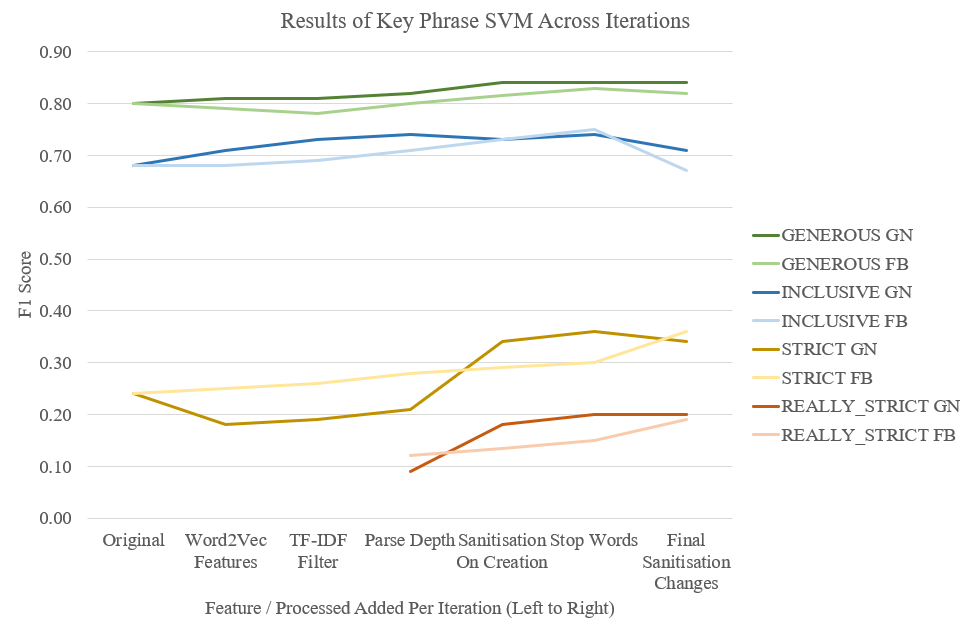
\includegraphics[width=\textwidth]{img/kpsvmresults.png}
	\caption[Key Phrase SVM Self Evaluation Through Iterations]{The key phrase SVM self evaluation results for varying strictness across iterations, where each iterations changes 1 thing. The coloured lines denote strictness as defined in table \ref{table:strictness}, with the legend assigning each colour to each strictness level. With each assignment, the darker of variant of the same colour is when the Google News (GN) Word2Vec model is used, and the lighter for when the Freebase (FB) model is used. Very strict evaluation was only created part way through development, so some early results are missing for that, but they would likely follow a similar patter to that of matching or \textit{strict} evaluation.}
	\label{figure:kpsvmresults}
\end{figure}

As described in the design section of this report, the SVM created for extracting key phrases began with a set of features which then underwent several iterations with other features and post processing being added. The full results, from start to finish, can be seen in figure \ref{figure:kpsvmresults}.

The results of the initial SVM are interesting. The strict metric shows middling results below that of ScienceIE's average. However, the two more generous metrics are very high. This implies two good things: Firstly, as the \textit{inclusive} metric is high, it shows that while some unwanted information is being extracted, much of the key phrase data is been chosen. Furthermore, the \textit{generous} metric scoring not too much higher implies that a lot of the other key phrases incorrectly extracted are just noise produced by the SVM rather than the gold key phrases with some missing information. This shows that the SVM isn't performing terribly as much of the required information is outputted, however, it has some overflowing of extra information which needs to be reduced. The redundant information could be removed by improvements to the SVM, as well as some post analysis and processing to remove extra, unwanted pieces of information, which is why the processes discussed above were developed and their analysis is to follow.

The Word2Vec features added generally slightly improved things across all metrics for at least one Word2Vec model. Oddly, while using the Google News model increased the score for the more generous two metrics, it negatively impacted the strict metric, reducing the F1 score by 6\% compared to the original score. The Freebase model was the opposite of this, although less significant differences were observed, as for the more generous metrics things slightly degraded, and for the strict metric things slightly improved. For this feature, it would imply Freebase was the best model to use as it did increase the results of the strictly measured predictions. 

The first post processing effect was added here with the TF-IDF filter. This gave all configurations minor improvements (the average F1 score rose by 0.01) as expected. 

Including the parse depth feature saw averagely 0.01 score improvements across the board as well. The graph showing progression also begins to include the very strict metric as well. This metric is in-line with how the ScienceIE evaluation works, matching both the key phrase string and position in the document. The result saw a 60\% score reduction compared to the, just string matching, strict metric when using both Freebase and Google News. This means the system is choosing useful pieces of information from the papers, but unfortunately roughly half of the key phrases chosen are not from the correct place in the text. 

Following this, the largest change to the SVM based key phrase extraction system happened; the inclusion of the \textit{sanitisation on creation} changes saw large improvements in F1 score - averagely 0.1 improvement for the Google News based strictly and very strictly evaluated tests. This was a very positive step, as the two generous metric scores didn't change very much. This mean that this post processing was effectively transforming a number of key phrases from being inclusive of the gold standard to matching the gold standard. 

Including the stop word flag feature again slightly improved things for the actual SVM performance, again averaging an increase of 0.01 F1 score.

The final change to the SVM process was to make the final changes to the key phrase creation sanitisation. While averagely this made no difference to the F1 results, for some cases it significantly damaged scores; namely when using the inclusive metric with the Freebase model, the F1 score dropped by almost 0.1. The Freebase model, under these presented set of features and processes, performs worse than the Google News model for all metrics aside from \textit{strict}, where the difference is only 0.02 F1 score. This change was still positive however, as it made the key phrases much more pleasant to look at. Cases such as "support vector machine (svm" was tidied up, and generally words were not missing final letters which was a problem from earlier in SVM's life. Furthermore, this last change saw an opportunity to quickly generate some synonyms for almost no cost. Using this method saw 14 synonyms correctly generated when processing the test data. 

From this, the best configuration can be seen to be when all proposed features and processing effects are used, with the Google News model being used for the Word2Vec features. Running this configuration and evaluating the predicted key phrase with the ScienceIE test scripts produces an overall F1 score of 0.2. This is perfectly in line with the self evaluation conducted under the strictest metric, which reinforces the self evaluation as trustworthy (as it got the correct score), and through that helps to validate claims the other evaluations give the information about the system they are meant to. 

\subsubsection{Experimenting With Longer Documents}
% TODO experinemnt with longer documents on paper...

\subsection{Method 2: Clustering}
While the SVM method showed some good results, unfortunately clustering was not as successful. 

A problem encountered during development was that not every word was in the Word2Vec vocabulary, meaning not every word could be clustered. This is actually quite a major problem as, given the context of the words we'd like to cluster is scientific papers, many of these unusual words not in the corpus are likely part of the key words describing the key pieces of information in the paper. Given we want to be able to cluster based on those terms to find them in future papers to extract as key phrases, this limits the capability and robustness of the algorithm. The only thing that could be done was to continue clustering until we are left with one cluster with everything that can be clustered in, and a group of clusters with one element each, where those singular terms are not in the vocabulary of Word2Vec. This problem didn't occur for every test paper processed, but has shown some papers to have over 20 tokens that were excluded from the Word2Vec model. 

Next came the problem of how the clusters formed. Ideally, we would like to see the case where, for many iterations, many clusters are present with many items each. This could then be used to split the document into many clusters with a (for instance) key phrase in each, taking the tokens at the centre of each cluster at a given level to be part of its own key phrase. What was generated instead was a pattern where, generally, two items clustered together which were there joined by a third item on the next iteration, then a fourth on the next, and so on, while no other tokens clustered together in other clusters. This is significantly less useful, as a bunch of words are grouped together in a growing group, while all others are left on their own until they are included in this large group. Very occasionally, other clusters grew to have a few items rather than immediately join the large cluster, but this was rare to see and still not very useful to draw multiple key phrases from.

To aid in the understanding of what happened, an illustration is provided in figure \ref{figure:kpclusteringeg}. The left drawing is the ideal case, and the right is what commonly occurred. It didn't necessarily have to happen in token order, but the point is that aside from picking tokens that are very close together, this does not give us much insight into the key topics of the paper.

\begin{figure}
	\centering
	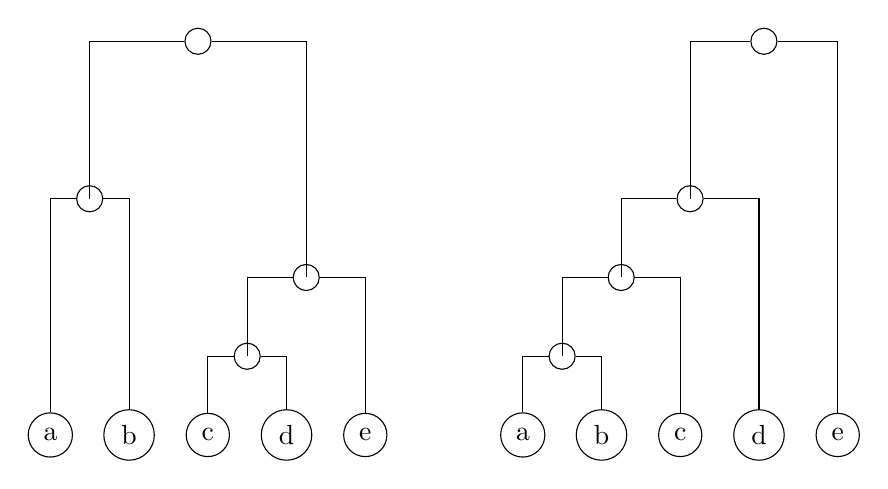
\begin{tikzpicture}[nodes={draw, circle}]
	\node (a) at (-4, 0) {a};
	\node (b) at (-3, 0) {b};
	\node (c) at (-2, 0) {c};
	\node (d) at (-1, 0) {d};
	\node (e) at (0, 0) {e};
	\node (ab) at (-3.5, 3) {};
	\node (cd) at (-1.5, 1) {};
	\node (cde) at (-0.75, 2) {};
	\node (all) at (-2.125, 5) {};
	
	\draw  (a) |- (ab);
	\draw  (b) |- (ab);
	\draw  (c) |- (cd);
	\draw  (d) |- (cd);
	\draw  (e) |- (cde);
	\draw  (cd.center) |- (cde);
	\draw  (ab.center) |- (all);
	\draw  (cde.center) |- (all);
	
	\node (a2) at (2 ,0) {a};
	\node (b2) at (3, 0) {b};
	\node (c2) at (4, 0) {c};
	\node (d2) at (5, 0) {d};
	\node (e2) at (6, 0) {e};
	\node (ab2) at (2.5, 1) {};
	\node (abc2) at (3.25, 2) {};
	\node (abcd2) at (4.125, 3) {};
	\node (all2) at (5.0625, 5) {};
	
	\draw  (a2) |- (ab2);
	\draw  (b2) |- (ab2);
	\draw  (c2) |- (abc2);
	\draw  (d2) |- (abcd2);
	\draw  (e2) |- (all2);
	\draw  (ab2.center) |- (abc2);
	\draw  (abc2.center) |- (abcd2);
	\draw  (abcd2.center) |- (all2);
	\end{tikzpicture}
	\caption[Visual Representation of Key Phrase Clustering]{Examples of hierarchical clustering on a set of items, \textit{a}, \textit{b}, \textit{c}, \textit{d} and \textit{e}, through to when they are all in the same cluster. The left drawing is an example of ideally what we would like to have seen. The right is a representation of what was very common generated.}
	\label{figure:kpclusteringeg}
\end{figure}

\section{Subtask B - Key Phrase Classification}

\begin{table}
	\centering
	\begin{tabular}{ C{2.5cm} | C{2cm} | C{2cm} | C{2cm} | C{2cm} | C{2cm} }
		\textbf{Word2Vec Model} & \textbf{Distance Metric} & \textbf{Default Class} & \textbf{Remove words?} & \textbf{Use many words?} & \textbf{Accuracy} \\
		\hline
		Google News & Average & Unknown & No & No & \textbf{47.90\%} \\
		Google News & Average & Unknown & Yes & No & \textbf{47.76\%} \\
		Google News & Average & Unknown & No & Yes & \textbf{45.47\%} \\
		Google News & Average & Unknown & Yes & Yes & \textbf{45.47\%} \\
		\textbf{Google News} & \textbf{Average} & \textbf{Material} & \textbf{No} & \textbf{No} & \textbf{54.58}\% \\
		Google News & Average & Material & Yes & No & \textbf{54.43\%} \\
		Google News & Average & Material & No & Yes & \textbf{52.14\%} \\
		Google News & Average & Material & Yes & Yes  & \textbf{52.14\%} \\
		Google News & Closest & Unknown & No & No & \textbf{46.05}\% \\
		Google News & Closest & Unknown & Yes & No & \textbf{45.96\%} \\
		Google News & Closest & Unknown & No & Yes & 44.05\% \\
		Google News & Closest & Unknown & Yes & Yes & 43.91\% \\
		Google News & Closest & Material & No & No & \textbf{52.73\%} \\
		Google News & Closest & Material & Yes & No & \textbf{52.63\%} \\
		Google News & Closest & Material & No & Yes & \textbf{50.73}\% \\
		Google News & Closest & Material & Yes & Yes & \textbf{50.58\%} \\
		Freebase & N/A & Unknown & N/A & N/A & 0.00\% \\
		Freebase & N/A & Material & N/A & N/A & 44.05\% \\
	\end{tabular}
	\caption[Word2Vec Classification Results]{The above table is the various configurations of the Word2Vec classifier, running with every possible configuration for the five parameters are listed. The result in bold line is the highest scoring configuration, with bold results being those above the baseline score of 44.05\% which is where every key phrase is simply classified as a \textit{material}. All Freebase results were not listed as there was no change in result other than for the \textit{default class} variable, so \textit{N/A} is present instead of each iteration of those variables. These results are based on classifying all 2052 ScienceIE key phrase test data points.}
	\label{table:classresults}
\end{table}

Key phrase classification under the outlined Word2Vec classifier was quick to execute. After the initial, one time per system boot, wait for the Word2Vec model to be loaded into memory, the actual calculations required are very fast to execute, giving this classifier a very high throughput.

In terms of result, it can be seen that several configurations allow for over 50\% of the key phrases to be classified correctly. The full range of results for each configuration can be seen on table \ref{table:classresults}.

The obvious thing to note here is that all tests under Freebase without a default class have a 0\% accuracy (i.e. it didn't classify any key phrase correctly). With a little investigation, if all key phrases were labelled as a \textit{material}, the accuracy would be 44\% - which is what was achieved by all configurations with the Freebase model and a default classification of \textit{material}. Therefore, Freebase clearly isn't an effective vocabulary for working with scientific publications, seemingly containing one of the supplied words. 

When using the Google News model, things are less clear. Generally, using this model a decent accuracy can be achieved, even without the support of a default classification. This shows the model does include many of the terms used in the publications presented. In terms of distance metric, \textit{average} was slightly better; it was part of the best configuration (scoring 54.6\%), and also the average of all of the \textit{average} distance configurations was 2\% higher than the average of the \textit{closest} configurations (50\% and 48\% respectively).

The configuration change that made the least difference was whether or not the unimportant and stop words were removed. This saw changes, averagely, of 0.1\% when comparing two configurations differing in only whether these words were removed. When some words were not removed the algorithm performed better, indicating that these words are more important than first thought for deciding class. This may be down to the edge cases discussed such as "He" or similar which, despite being a stop word, we would want to keep.

Using various words when finding similarity decreased the accuracy of classification, and was the largest detrimental parameter. When using many words to find similarity, accuracy decreased an average of 2.2\% (50.3\% down to 48.1\%). This means the position of the target classes in the Word2Vec model are likely quite accurate when compared to words that can be used in a similar context.

Using the best configuration found my testing within this paper, evaluating this classifier through the ScienceIE scripts gives an F1 score of 0.55 when evaluated individually (given the gold standard key phrases). This isn't a bad score, as it almost matches the average ScienceIE F1 score for this section done independently.

\subsection*{Other Experimentation}
While working on key phrase classification, having seen some decent results produced by the SVM created in subtask 1, a short experiment was conducted to see how well using position in a document could be used to determine classification.

The process of trying this was very simple: re-purpose the subtask A SVM (with all described extensions included) code to, when training, label data according to a class rather than to key phrase. Two versions of this were attempted:

\begin{itemize}
	\item The SVM is given 4 different labels, one for each classification and one for no classification (i.e. not part of a key phrase).
	\item 3 different SVMs were trained, each only having one classification labelled.
\end{itemize}

Given the only real semantic meaning for a token in the SVM was based around whether the token was a noun, this was not expected to perform well as semantics and the specific words surrounding what we are trying to classify generally are expected to be important, rather than the position of the token in the text which gives us little context.

As expected, results were terrible, with F1 scores for both versions being less than 0.1. This confirms that the position of tokens, at least as far as this paper's positional information is concerned, is not useful in classifying tokens. It may have been interesting to try again leaving out non key phrase tokens from the training data generated for the SVM to learn from, but these low results didn't encourage further study into this idea when other, more efficient and productive concepts were being worked on.

\section{Subtask C - Relation Extraction}

Both SVMs concepts were tested and the results for the hyponym and synonym variants combined for full evaluation.

\begin{table}
	\centering
	\begin{tabular}{c | c | c | c | c }
		\textbf{SVM Model} & \textbf{Vector Generation} & \textbf{True Positives} & \textbf{False Positives} & \textbf{F1 Score} \\
		\hline
		\textit{Many Features} & All tokens included & 13 & 84 & \textbf{0.09} \\
		\textit{Many Features} & Root noun selected & 2 & 28 & 0.02 \\
		\textit{Many Features} & Unimportant words removed & 0 & 0 & 0 \\
		\textit{Few Features} & All tokens included & 0 & 0 & 0 \\
	\end{tabular}
	\caption[Relation Extraction Specific Results]{Results from doing relation extraction with the proposed SVMs. The results are calculated after the relations extracted by the hyponym and synonym SVMs are combined. The \textit{vector generation} column described how a vector for a key phrase was found (for example, where the unimportant words are removed). The bold result is the highest F1 score achieved.}
	\label{table:relresults}
\end{table}

As presented in summary table \ref{table:scienceieresults}, the best overall results for this synonym extraction was an F1 score of 0.1\%. This was from using the \textit{many features} SVM with the vectors from each token in a key phrase being used to calculate a key phrases total vector. A more detailed breakdown of how well each configuration performed can be seen in table \ref{table:relresults}. 

From this table is it clear to see that the \textit{many features} SVM concept performed better than the \textit{few features}. While the hope was to allow the SVM to work on information with a lower complexity to help it find a better fitting hyperplane, this clearly hasn't worked as it didn't pick any relations at all; compared to \textit{many features} with the same vector generation, which chose a total of 101 relations. 

In terms of the different methods of generating vectors for key phrases, keeping all of the information in the key phrase appears to be the best method. Most true positives where found when all tokens are kept, while less true positives came from where the root nouns are selected, and no true positives were found when stop words and unimportant words were removed. This mirrors what happened in subtask B, where potentially unimportant information was removed and a decrease in the quality of results is observed; although it is more noticeable here given it is the difference between some and no relations being extracted (there was only a 0.1\% change in subtask B's results).

Furthermore, while leaving more important information in the key phrase for vector generation did improve the system performance, the false positives increases a large amount as well. Selecting just the root noun saw 14 times more false positive results than true positive; compared to when all key phrase information was left in, only 6 times as many false positives to true positives were seen. Not excluding data clearly improves the system accuracy, and increases the F1 score.

\section{Conclusion}
This paper set out to provide a set of solutions to the ScienceIE task and its subtasks. Considering the summary presented in table \ref{table:scienceieresults}, these experimental systems have performed in a satisfactory manor. 

The key phrase extraction, using a range of features in a support vector machine and some effective post processing achieved reasonable results considering, if we ignore the location of the key phrase extractions, a maximum F1 score of 0.36 which is very close the to average at ScienceIE. For comparisons sake, it would be very interesting to run the same analysis on the results produced at ScienceIE, to see if the best teams realistically came very close to extracting 100\% of the required information (if the position of key phrases could be ignored, and potentially a little bit of extra information allowed).

The key phrase classification produced good results, again being very close to the average at ScienceIE. While the Freebase Word2Vec model did not serve this use well, the Google News model did a very good job of classifying key phrases, producing comparable results with or without a default classification to give if it couldn't understand a key phrase. 

Finally, the relation extraction did not perform very well, even when attempting just hyponym or synonym extraction. In fact, the one simple rule included in the post processing for subtask A produced 1 more correct synonym than any synonym SVM did during testing with gold standard data as an input. From this, unfortunately using just Word2Vec as a basis for a SVM feature set cannot be recommended, as it has very poor performance under these conditions. It is believe, however, that part of this is because of the lack of testing data as input, given there were many examples given to the SVM of what a relationship didn't look like, where there were few examples of what the relationships did look like.

\subsection{Improvements}
From this, a range of improvements and extensions could be applied:
\begin{itemize}
	\item \textbf{A more appropriate Word2Vec model.} Word2Vec was used in all three subtasks, but unfortunately only two models were tested with the systems, and neither had the context of scientific papers. If a system was created to crawl the internet fetching many scientific publications and have them all processed by Word2Vec, there may be a potential for a more suitable model to be created. Not only would the vocabulary be laid out in vector space in a way that should likely fit the testing data presented here better, but more of the tokens in this testing data should also appear in the model, which would improve things significantly for a start. 
	\item \textbf{Expansion of key phrase SVM features.} If future work was to continue on the SVM created in subtask A, a way that is likely to produce better results is to include more features about each token. Specifically:
	\begin{itemize}
		\item Features giving more information about surrounding key phrase tokens (for example more information about recent key phrase tokens, information about overall key phrases so far for the given document),
		\item The Word2Vec distance to the previous token (in an attempt to string together related tokens),
		\item More lexical or semantic information about the current phrase.
	\end{itemize}
	\item \textbf{More training time and memory capacity for parameter tuning.} Time and memory limitations didn't allow for much more training time to be given to the \textit{many features} SVM, but potentially an increased \textit{C} value may help to find a hyperplane which could work better. For the key phrase SVM, while the parameters tested in cross validation seemed to plateau, further investigation may have revealed increased performance.
	\item \textbf{Better data for training the relation SVMs.} As alluded to above, give the relation SVMs training data which includes a higher percentage of actual relations cases. This could be done through adding more papers with relations in, or removing some or all papers without any relations in.
\end{itemize}

\pagebreak
\chapter{Creating a Proof of Concept Use for ScienceIE data}
\section{Concept and Specification}
Having completed systems to handle the information extraction, the next major part of the project was to explore how this information can be utilised for researchers. 

The most obvious domain for using summary information about a set of resources is search. Being able to efficiently search through a large set of documents to quickly find more useful information is a very useful thing. The focus of this section is to explore using the key phrase information in an efficient and convenient way to aid in user query across the ScienceIE data set. 

The ScienceIE data set is specifically being used because that is what the algorithms in this project are designed for. The problem of handling longer, full publications has been discussed, so to not complicate this investigation further, the standard short documents of ScienceIE shall form the database of documents.

The following requirements are presented for the POC system to conform to are:
\begin{enumerate}
	\item As a basis to make the system usable, the ability to list papers in the database, and the ability to present all the information about a paper on one screen. The ability to download the extractions in the BRAT format should also be made available. 
	\item A search system for the key phrase information gained. This should allow the input of a user query (plain natural language text), with an option to give some indication of the classification of the information they are interested in (i.e. \textit{task}, \textit{process} or \textit{material}).
	\item The ability to add papers dynamically to the database throughout run time. This means not only should the system support the creation of new paper records, but also the automatic processing of that paper through all 3 subtasks of ScienceIE, with the results being available to the search system.
	\item Some way of conveying summary information about the extractions contained in the system. While not essential for search, having a convenient way for the developer and users to take a snapshot of what is contained in the system is useful for evaluation purposes, including giving an indication of how many papers are included and their processing status.
\end{enumerate}

\section{Background and Technology Review}
\subsubsection*{Existing Search}
Two popular, publicly available search engines have been examined to extra some well designed features from. These are Google Scholar\footnote{\href{https://scholar.google.com/}{https://scholar.google.com/}} and ScienceDirect\footnote{\href{https://www.sciencedirect.com/}{https://www.sciencedirect.com/}}, and appendix \ref{appendix:searcheg} shows screen shots of both web sites given the same query. Common features are:
\begin{itemize}
	\item Limited results per page (10 on Google Scholar, 25 on ScienceDirect),
	\item The total number of documents selected and the time it took to do this is displayed to the user,
	\item Filtering options, including by date,
	\item The title of a result is followed by a snippet of the document, with relevant words highlighted in some way,
	\item The title is a link to an individual results page which presents information about the document, but there are also links to directly get the document downloaded.
\end{itemize}

\noindent Some custom features on each website are:
\begin{itemize}
	\item ScienceDirect supports searches with multiple parameters, including query fields specifically for author, title, pages, etc...
	\item ScienceDirect also supports custom numbers of search results per page; 25 is the default, but the user can receive 50 or 100 results per page if they wish,
	\item Google Scholar present \textit{related searches} to allow the user to navigate sideways towards their target paper, rather than straight down to it,
	\item ScienceDirect features a \textit{recommended} section at the top where it showcases several publications it believes to be the most relevant.
\end{itemize}

Given the data set available in this project, most of these ideas presented by Google Scholar and ScienceDirect can be implemented. However, as ScienceIE's data is purely text snippets of documents, author, real title, publish information and more are unavailable, meaning any system created here cannot support filtering by these features, or display that information. An original hope of the developer was to include a more advanced search, potentially including a PageRank type system \cite{Page1998} where the links would be based on referencing, but unfortunately without even the reference information for each paper available, this is impossible to achieve whit the ScienceIE dataset.

The search on these two websites is likely be based on latent semantic analysis (\cite{Landauer1998} and \cite{AswaniKumar2012}) which looks at the similarities between search terms and attempts to take into account context. This method of representing words in a vector space prepared for querying is a popular method of document retrieval. This method of querying could potentially be modified to involved more weighting of tokens if the are included in key phrases, or be used to inspire a new algorithm that uses key phrase information to help with weighting word importance.

\subsubsection*{Available Technologies}
The goal with this project is to prove a use of the data produced as part of ScienceIE through some application. To make this application available for use, a web based service will be created that allows any user to join without the need for complex setup. The benefits of this include not having to distribute installation media and update media, along with centralised management of any database of information and being able to immediately make available new features.

In terms of storing information, popular database technologies were surveyed. The stack overflow survey 2017 listed MySQL\footnote{\href{https://www.mysql.com/}{https://www.mysql.com/}} as the most used SQL platform by developers on the sight\footnote{\href{https://insights.stackoverflow.com/survey/2017\#technology-databases}{https://insights.stackoverflow.com/survey/2017\#technology-databases}}. One reason for this is that some competitive SQL platforms require licensing (especially when commercial use is considered), such as Oracle SQL, while MySQL is open source and can be used more freely. The platform can be easily acquired and installed on various platforms (with major Windows and Linux operating systems supported), with largely straight forward initial configuration (for a project of this scale). The standard MySQL installation also includes the MySQL Workbench, which includes a convenient tool for building a relational database schema\footnote{\href{https://dev.mysql.com/doc/workbench/en/wb-data-modeling.html}{https://dev.mysql.com/doc/workbench/en/wb-data-modeling.html}}, with the ability to export SQL scripts to build the designed database in a single execution (including tables, relations and users with certain access rights). 

One of the most popular Java web frameworks available is Spring. Spring provides functionality to route requests to certain Java classes for processing, including the passing of any parameters with some degree of automatic validation, and the ability to process Java Servlet Pages (JSPs) which are compiled at run time to delivery varying pieces of information to the end users. It implemented the standard \textit{model-view-controller} (MVC) design pattern. To keep the focus on the use of data processed in this project, a convenient web container is desired, and that is what Spring Boot\footnote{\href{https://projects.spring.io/spring-boot/}{https://projects.spring.io/spring-boot/}} provides. This packages the Spring technology stack, web server technology (for example, Apache Tomcat) and any extra libraries required into a single, executable, Java project, making heavy use of annotations for the minimal configuration required. This makes it an extremely portable and (in terms of environment and system configuration) light weight application to set-up and run, which reflects as part of their projects mission statement to get developers "up and running as quickly as possible". It is a young project, with the original version being released in 2014 and version 2.0 being released during the course of this project, meaning it is built to work with the current standard of industrial Java technologies - so while this project is aiming to build a simple application, it shall have some powerful technologies standing behind it.

% TODO find a reference for MVC?

One of these technologies is Hibernate\footnote{\href{http://hibernate.org/}{http://hibernate.org/}}. This integrates with the Java Persistance API (JPA), supported by Spring, for extremely simply database interactions with many functions being supported by default. It combines a simple Java object which holds fields relating to each of the column in a database entity (table), and an abstract \texttt{CrudRepository} class which can be extended from to make a data access object which can retrieve records from a database and update them as well. Methods can be added to the extended class to make more complex queries, and either plain English can be used in the method name to define the query, or the specific SQL query statement can be specified if required\footnote{A guide to using this technology is freely available on Spring's website and is presented in a very simple manor. It can be viewed at \href{https://spring.io/guides/gs/accessing-data-jpa/}{https://spring.io/guides/gs/accessing-data-jpa/}} Furthermore, when fields are foreign keys of other entities, rather than being of an \textit{ID} type such as \texttt{Integer} or \texttt{Long}, the class representation of the foreign entity can be used instead, and Hibernate will automatically populate it with the correct object.

\section{Design and Configuration}

\subsection*{Design of the Services}
There are four key requirements of the POC system which cover a large amount of usability. The first requirement is very simple. Two pages are required for this:
\begin{itemize}
	\item The first is simply a list of papers, each selectable. When selected, the user will be taken to the next paper described.
	\item The second page, for displaying information about a paper, should begin with the title at the top, a section in the middle for the original text, and finish with a list of key phrases and relations. The key phrases, as a minimum, should be annotated on the main text as well.
\end{itemize}

The second requirement is covering the question of search. A new algorithm is proposed that includes the key phrase information about a paper. Using the concept of using the TF-IDF scores of both the tokens in all documents as well as the tokens in the query to try to find papers is utilised with a scaling factor, defined by the presence of key words in a paper.

\subsection*{Database Design and Entity Relationship Diagram}

\begin{figure}
	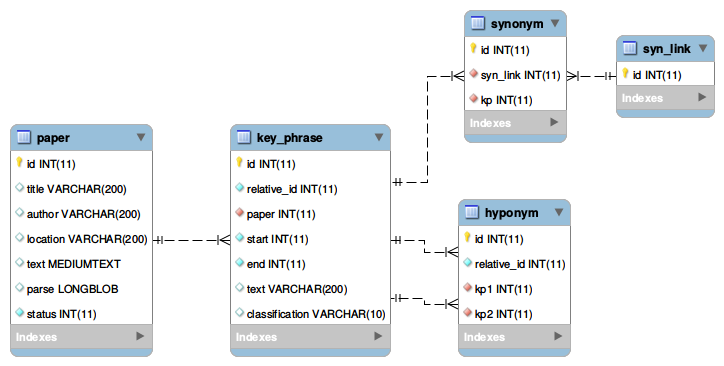
\includegraphics[width=\textwidth]{img/fypdberd.png}
	\caption[Database Entity Relationship Diagram]{The entity relationship diagram that supports this proof-of-concept system, as exported from the MySQL Workbench tool kit. Primary keys are represented by gold keys, foreign keys are red diamonds, normal fields are blue diamonds and hollow blue diamonds indicate the field is nullable. Types for all fields in all entities are also shown. The Java representation of these entities share the same name in all cases, converted to camel case, aside from the entity titles which have \texttt{DAO} appended (standing for \textit{data access object}) as without this the class names would clash with those used in the NLP system, which would have been confusing to program with. As examples, the \texttt{paper} entity was \texttt{PaperDAO} in the Java project, but an \texttt{id} field would remain \texttt{id} in the Java code to follow the standard.}
	\label{figure:dberd}
\end{figure}

The support storage and query of the data produced by the ScienceIE task, a suitable database must be designed and created. Given a lot of the required entities had been created as part of the NLP system, the data base design heavily inherits the classes and fields from this. The full design for the database is shown in figure \ref{figure:dberd}

The \texttt{paper} and \texttt{key\_phrase} entities are largely the same as their equivalents in the NLP system. Of course, rather than having a list of key phrases held within the \texttt{paper} entity, the \texttt{key\_phrase} entity has a field to store a reference to its parent \texttt{paper}. The \texttt{paper} entity also has two fields no in the NLP system: a \texttt{status} which was discussed above, and a \texttt{parse} which holds a serialised \texttt{Paper} Java object. This allows the preprocessing to take place and for that information to be stored directly in the database with its parent record, removing the need for re-computation of preprocessing every time the paper is called from the database.

The method for storing hyponyms and synonyms is slightly different to the NLP system. Rather than being part of a relations list the parent paper record holds, instead each relation holds the \texttt{key\_phrase} references they are a relation of. The original \texttt{paper} can still be retrieved through retrieving the referenced \texttt{key\_phrase} records. The \texttt{hyponym} record holds the two \texttt{key\_phrase} records it is a relation of, as well as a relative ID, which is the ID of the hyponym relation relative to the individual paper it is from. The \texttt{synonym} relation is a little more complex. While the NLP system created didn't support more than two way synonym relation extraction and there was only one example of a three way synonym relation in the ScienceIE data set, to support the range of relations defined as part of ScienceIE these synonym entity has to support one synonym referencing a variable amount of \texttt{key\_phrase} records. Therefore, to avoid a many-to-many relation between entities, each \texttt{synonym} record holds a reference to a \texttt{syn\_link}, the concept being a set of synonyms, each referencing one \texttt{key\_phrase}, all reference the same \texttt{syn\_link} record, which makes the synonym relation between the set of referenced key phrases. Having \texttt{syn\_link} also provides a convenient way to count he number of synonyms in the system.

\section{Implementation}

\subsection*{Project Configuration}
The creation of the project involved including various dependencies in the \texttt{pom.xml} file and setting up the launch configuration for Spring Boot.

To include Spring Boot, \texttt{pom.xml} was configured as described on the Spring Boot website, along with a connector package for MySQL\footnote{\href{https://spring.io/guides/gs/accessing-data-mysql/}{https://spring.io/guides/gs/accessing-data-mysql/}}. 

\begin{figure}
	\begin{lstlisting}[language=XML]
<dependency>
  <groupId>xyz.tomclarke.fyp</groupId>
  <artifactId>fyp-nlp</artifactId>
  <version>0.0.1-SNAPSHOT</version>
  <!-- Stop logging dependency errors -->
  <exclusions>
    <exclusion>
      <groupId>ch.qos.logback</groupId>
      <artifactId>logback-core</artifactId>
    </exclusion>
    <exclusion>
      <groupId>org.slf4j</groupId>
      <artifactId>slf4j-log4j12</artifactId>
    </exclusion>
  </exclusions>
</dependency>
	\end{lstlisting}
	\caption[Configuration to set the NLP system as a dependency in Maven]{The Maven configuration for listing the NLP project as a dependency, as used in the POC system. Note, the exclusion (as discussed) are to remove logging dependency conflicts using Spring Boot causes; this may break logging if another system uses this configuration but doesn't have its own logger available.}
	\label{figure:nlpdependency}
\end{figure}

To use the NLP system built in this project, Maven also needed to be told to import this so it can be used to generate information about given papers when the full system has been developed. Given the NLP system has been compiled and installed to the local Maven repository (as it is not hosted anywhere), the configuration shown in figure \ref{figure:nlpdependency} will include the NLP system in a compiled project. Doing this also sets any dependencies of the NLP system as dependencies of this system, so they do not need to be re-listed as dependencies. The unfortunate effect of this is where there are conflicts between dependencies, which is what happened in this project. The logging included in Spring Boot was an alternate version to that in the NLP project, and while it didn't damage any part of the system, on every boot it would choose one of the loggers and print out many error messages warning the developer against it. Therefore, the conflicting dependencies in the NLP system were excluded to remove this problem, and this was done to the NLP system rather than to Spring Boot as this problem may occur if the NLP system was used in another project including other dependencies, so it made sense to list how to fix it for the NLP system dependency. 

For the system to launch, some basic configuration had to be set. There is an \texttt{application.properties} file in the Java resources with the following parameters (with explanations as to why those were chosen appended):
\begin{itemize}
	\item \texttt{server.port=8080} 8080 is a standard port for testing web applications on. Furthermore, port 80 needs administrative privileges to be used ever time the application is launched, which would not only be frustrating to a developer, but not supporting good security standards if there was a vulnerability in the web service. The router the developer system was sitting behind, through port forwarding, allowed incoming connections on port 80 to be directed to 8080 on the developer system, so when connecting via web browser, no port would be needed to be specified.
	\item \texttt{debug=false} If \texttt{true} was set, this would output all debug information to the console. Given the log4j configuration being used output all debug information to disk, there was no need to have it also in console, making it harder to see what was going on while running.
	\item \texttt{spring.jpa.hibernate.ddl-auto=none} This parameter has several different possible values. \texttt{none} means the connection to the database is standard, allowing the Java application to commit reads and writes. Other values were possible, which would support (if the database hasn't been setup) automatic configuration of the database based on the entity declarations. While this could have been useful, control of configuring the database being left to the entity relationship software included in the MySQL workbench seemed preferable.
	\item \texttt{spring.datasource.url=\newline jdbc:mysql://tomclarke.xyz:3306/fyp?verifyServerCertificate=false\&useSSL=true} This is the JDBC connection string, allowing the system to find and connect to the database. To increase security, encryption of the connection through Secure Sockets Layer (SSL) is enabled, but as the database server is not configured with any certificate, this is set to be ignored.
	\item \texttt{spring.datasource.username=fyp\_user} This is simply the database user setup for the system to use. The permissions on this user were restricted to read and write of data in the \texttt{fyp} database, so if the application is compromised the database connection can't be used to read information from other databases on the same instance, or change the configuration of the database system. 
	\item \texttt{spring.datasource.password=$<$password$>$} This is the password of the database user for the system to login with.
\end{itemize}

Several parts of the above are concerned with, as well as required configuration, security of the database and system as whole, and while this project is not concerned with security, it is seen as good practise to include these features.

Finally, the class \texttt{FypGuiApplication} needed to be created, as it is this class that contains the classic \texttt{public static void main(String[] args)} method that starts the whole program. Along side the opportunity to include any other pieces of configuration completed through Java code, this initiated the Spring MVC technology stack.

\section{Web Interface}

\section{Testing}

\section{Conclusion}

\pagebreak
\chapter{Conclusion}
Overall, the solutions presented to the ScienceIE problem do not succeed in beating the solutions proposed as part of the task, however, do explore other ideas about how to achieve the goals. Word2Vec usage in particular was explored and utilised through the solutions provided to all three subtasks. A more suitable model for Word2Vec would have been useful and likely boosted the performance of the systems. The reason for creating these systems is to extract classified key pieces of information from scientific papers, and a use for this was proposed and demonstrated in the proof-of-concept website produced. This used key phrase information when completing search to try to prioritise relevant papers to a users query, which was reasonably fast and accurate, given the data available. 

The project was completed on time and mostly in accordance with the initial project plan. Small iterative improvements were constantly made to the code base through out, but periods of significant effort for various tasks is shown in the Gantt chart in figure \ref{figure:progresschart}.

\begin{figure}[H]
	\centering
	\begin{ganttchart}[y unit title=0.4cm,
		y unit chart=0.5cm,
		vgrid,hgrid, 
		title label anchor/.style={below=-1.6ex},
		title left shift=.05,
		title right shift=-.05,
		title height=1,
		bar/.style={fill=gray!50},
		incomplete/.style={fill=white},
		progress label text={},
		bar height=0.7,
		group right shift=0,
		group top shift=.6,
		group height=.3]{1}{21}
		% Labels
		\gantttitle{2017}{12}
		\gantttitle{2018}{9} \\
		\gantttitle{September}{3} % 3
		\gantttitle{October}{3} % 6
		\gantttitle{November}{3} % 9
		\gantttitle{December}{3} % 12
		\gantttitle{January}{3} % 15
		\gantttitle{February}{3} % 18
		\gantttitle{March}{3} \\ % 21
		% Tasks
		\ganttbar[bar/.append style={fill=green}]{Initial Research}{1}{5} \\
		\ganttbar[bar/.append style={fill=yellow}]{Project Configuration}{5}{5} \\
		\ganttbar[bar/.append style={fill=red}]{Library Exploration}{5}{6} \\
		\ganttbar[bar/.append style={fill=red}]{Subtask A SVM}{6}{11} \\
		\ganttbar[bar/.append style={fill=red}]{Subtask A Clustering}{9}{10} \\
		\ganttbar[bar/.append style={fill=red}]{Subtask C \textit{Many Features}}{10}{12} \\
		\ganttbar[bar/.append style={fill=red}]{Subtask B}{11}{12} \\
		\ganttbar[bar/.append style={fill=blue}]{POC Configuration Setup}{12}{12} \\
		\ganttbar[bar/.append style={fill=green}]{POC Research}{12}{15} \\
		\ganttbar[bar/.append style={fill=blue}]{POC Architecture}{13}{14} \\
		\ganttbar[bar/.append style={fill=blue}]{POC Screens}{14}{15} \\
		\ganttbar[bar/.append style={fill=blue}]{POC Services}{16}{18} \\
		\ganttbar[bar/.append style={fill=red}]{Subtask C \textit{Few Features}}{18}{18} \\
		\ganttbar[bar/.append style={fill=blue}]{POC Testing}{19}{19} \\
		\ganttbar[bar/.append style={fill=yellow}]{Miscellaneous Fixing}{20}{21}
	\end{ganttchart}
	\caption[Gantt Chart of Development]{A Gantt chart displaying the development progress of the project. The colours red, blue, green and yellow represent work on the NLP system, the POC system, research and miscellaneous tasks respectively. This roughly matches the initial project plan, although work on labelled sections was not fully exclusive (for example the subtask A SVM could be revisited to be improved upon while working on a POC task).}
	\label{figure:progresschart}
\end{figure}

\pagebreak

%----------------------------------------------------------------------
% References and Appendicies

\pagebreak
\bibliographystyle{agsm}
\bibliography{fyp.bib}

\pagebreak
\begin{appendices}
\appendix

\chapter{Example ScienceIE Training/Test Document}
\label{appendix:egpaper}
The following is ScienceIE test paper file S0010938X15301268.txt:\\

\noindent Fig. 9 displays the growth of two of the main corrosion products that develop or form on the surface of Cu40Zn with time, hydrozincite (Fig. 9a) and Cu2O (Fig. 9b). It should be remembered that both phases were present already from start of the exposure. The data is presented in absorbance units and allows comparisons to be made of the amounts of each species between the two Cu40Zn surfaces investigated, DP and HZ7. The tendency is very clear that the formation rates of both hydrozincite and cuprite are quite suppressed for Cu40Zn with preformed hydrozincite (HZ7) compared to the diamond polished surface (DP). In summary, without being able to consider the formation of simonkolleite, it can be concluded that an increased surface coverage of hydrozincite reduces the initial spreading ability of the NaCl-containing droplets and thereby lowers the overall formation rate of hydrozincite and cuprite.

\chapter{Example ScienceIE Training/Test Annotation Data}
\label{appendix:egann}
The following is ScienceIE test paper annotations file S0010938X15301268.ann:\\

\noindent T1	Material 46 64	corrosion products
T2	Material 104 110	Cu40Zn\\
T3	Material 122 134	hydrozincite\\
T4	Material 149 153	Cu2O\\
T5	Material 378 384	Cu40Zn\\
T6	Material 408 410	DP\\
T7	Material 415 418	HZ7\\
T8	Material 530 536	Cu40Zn\\
T9	Material 552 564	hydrozincite\\
T10	Material 566 569	HZ7\\
*	Synonym-of T9 T10\\
T11	Material 587 611	diamond polished surface\\
T12	Material 613 615	DP\\
*	Synonym-of T11 T12\\
T13	Material 678 691	simonkolleite\\
T14	Material 751 763	hydrozincite\\
T15	Material 809 833	NaCl-containing droplets\\
T16	Material 883 895	hydrozincite\\
T17	Material 900 907	cuprite\\
T18	Process 456 471	formation rates\\
T20	Process 280 296	absorbance units\\
T19	Task 308 406	comparisons to be made of the amounts of each species between the two Cu40Zn surfaces investigated\\
R1	Hyponym-of Arg1:T3 Arg2:T1\\
R2	Hyponym-of Arg1:T4 Arg2:T1\\
T21	Material 480 492	hydrozincite\\
T22	Material 497 504	cuprite\\
T23	Process 665 691	formation of simonkolleite\\
T24	Process 776 793	initial spreading\\
T25	Process 865 879	formation rate\\

\chapter{Stop Words List}
\label{appendix:stopwords}
Below is the list of stop words used in this project:\\
\begin{multicols}{7}
\noindent !!\\
?!\\
??\\
!?\\
`\\
``\\
''\\
-lrb-\\
-rrb-\\
-lsb-\\
-rsb-\\
,\\
.\\
:\\
;\\
"\\
'\\
?\\
$<$\\
$>$\\
\{\\
\}\\
$[$\\
$]$\\
+\\
-\\
(\\
)\\
\&\\
\%\\
\$\\
@\\
!\\
\^\\
\#\\
*\\
..\\
...\\
'll\\
's\\
'm\\
a\\
about\\
above\\
after\\
again\\
against\\
all\\
am\\
an\\
and\\
any\\
are\\
aren't\\
as\\
at\\
be\\
because\\
been\\
before\\
being\\
below\\
between\\
both\\
but\\
by\\
can\\
can't\\
cannot\\
could\\
couldn't\\
did\\
didn't\\
do\\
does\\
doesn't\\
doing\\
don't\\
down\\
during\\
each\\
few\\
for\\
from\\
further\\
had\\
hadn't\\
has\\
hasn't\\
have\\
haven't\\
having\\
he\\
he'd\\
he'll\\
he's\\
her\\
here\\
here's\\
hers\\
herself\\
him\\
himself\\
his\\
how\\
how's\\
i\\
i'd\\
i'llv
i'm\\
i've\\
if\\
in\\
into\\
is\\
isn't\\
it\\
it's\\
its\\
itself\\
let's\\
me\\
more\\
most\\
mustn't\\
my\\
myself\\
no\\
nor\\
not\\
of\\
off\\
on\\
once\\
only\\
or\\
other\\
ought\\
our\\
ours\\
ourselves\\
out\\
over\\
own\\
same\\
shan't\\
she\\
she'd\\
she'll\\
she's\\
should\\
shouldn't\\
so\\
some\\
such\\
than\\
that\\
that's\\
the\\
their\\
theirs\\
them\\
themselves\\
then\\
there\\
there's\\
these\\
they\\
they'd\\
they'll\\
they're\\
they've\\
this\\
those\\
through\\
to\\
too\\
under\\
until\\
up\\
very\\
was\\
wasn't\\
we\\
we'd\\
we'll\\
we're\\
we've\\
were\\
weren't\\
what\\
what's\\
when\\
when's\\
where\\
where's\\
which\\
while\\
who\\
who's\\
whom\\
why\\
why's\\
with\\
won't\\
would\\
wouldn't\\
you\\
you'd\\
you'll\\
you're\\
you've\\
your\\
yours\\
yourself\\
yourselves\\
\#\#\#\\
return\\
arent\\
cant\\
couldnt\\
didnt\\
doesnt\\
dont\\
hadnt\\
hasnt\\
havent\\
hes\\
heres\\
hows\\
im\\
isnt\\
its\\
lets\\
mustnt\\
shant\\
shes\\
shouldnt\\
thats\\
theres\\
theyll\\
theyre\\
theyve\\
wasnt\\
were\\
werent\\
whats\\
whens\\
wheres\\
whos\\
whys\\
wont\\
wouldnt\\
youd\\
youll\\
youre\\
youve\\
\end{multicols}

\chapter{Google Scholar and ScienceDirect Search Pages}
\label{appendix:searcheg}
The following are screen shots of the query "computer science" being queried in two popular search engines: Google Scholar (left) and ScienceDirect (right). The "\textbf{$\cdot$$\cdot$$\cdot$}" denote some of the search results has been cropped out. As cropping has been applied, the results presented by Google Scholar and ScienceDirect are 10 and 25 (configurable to 50 or 100) respectively. \\

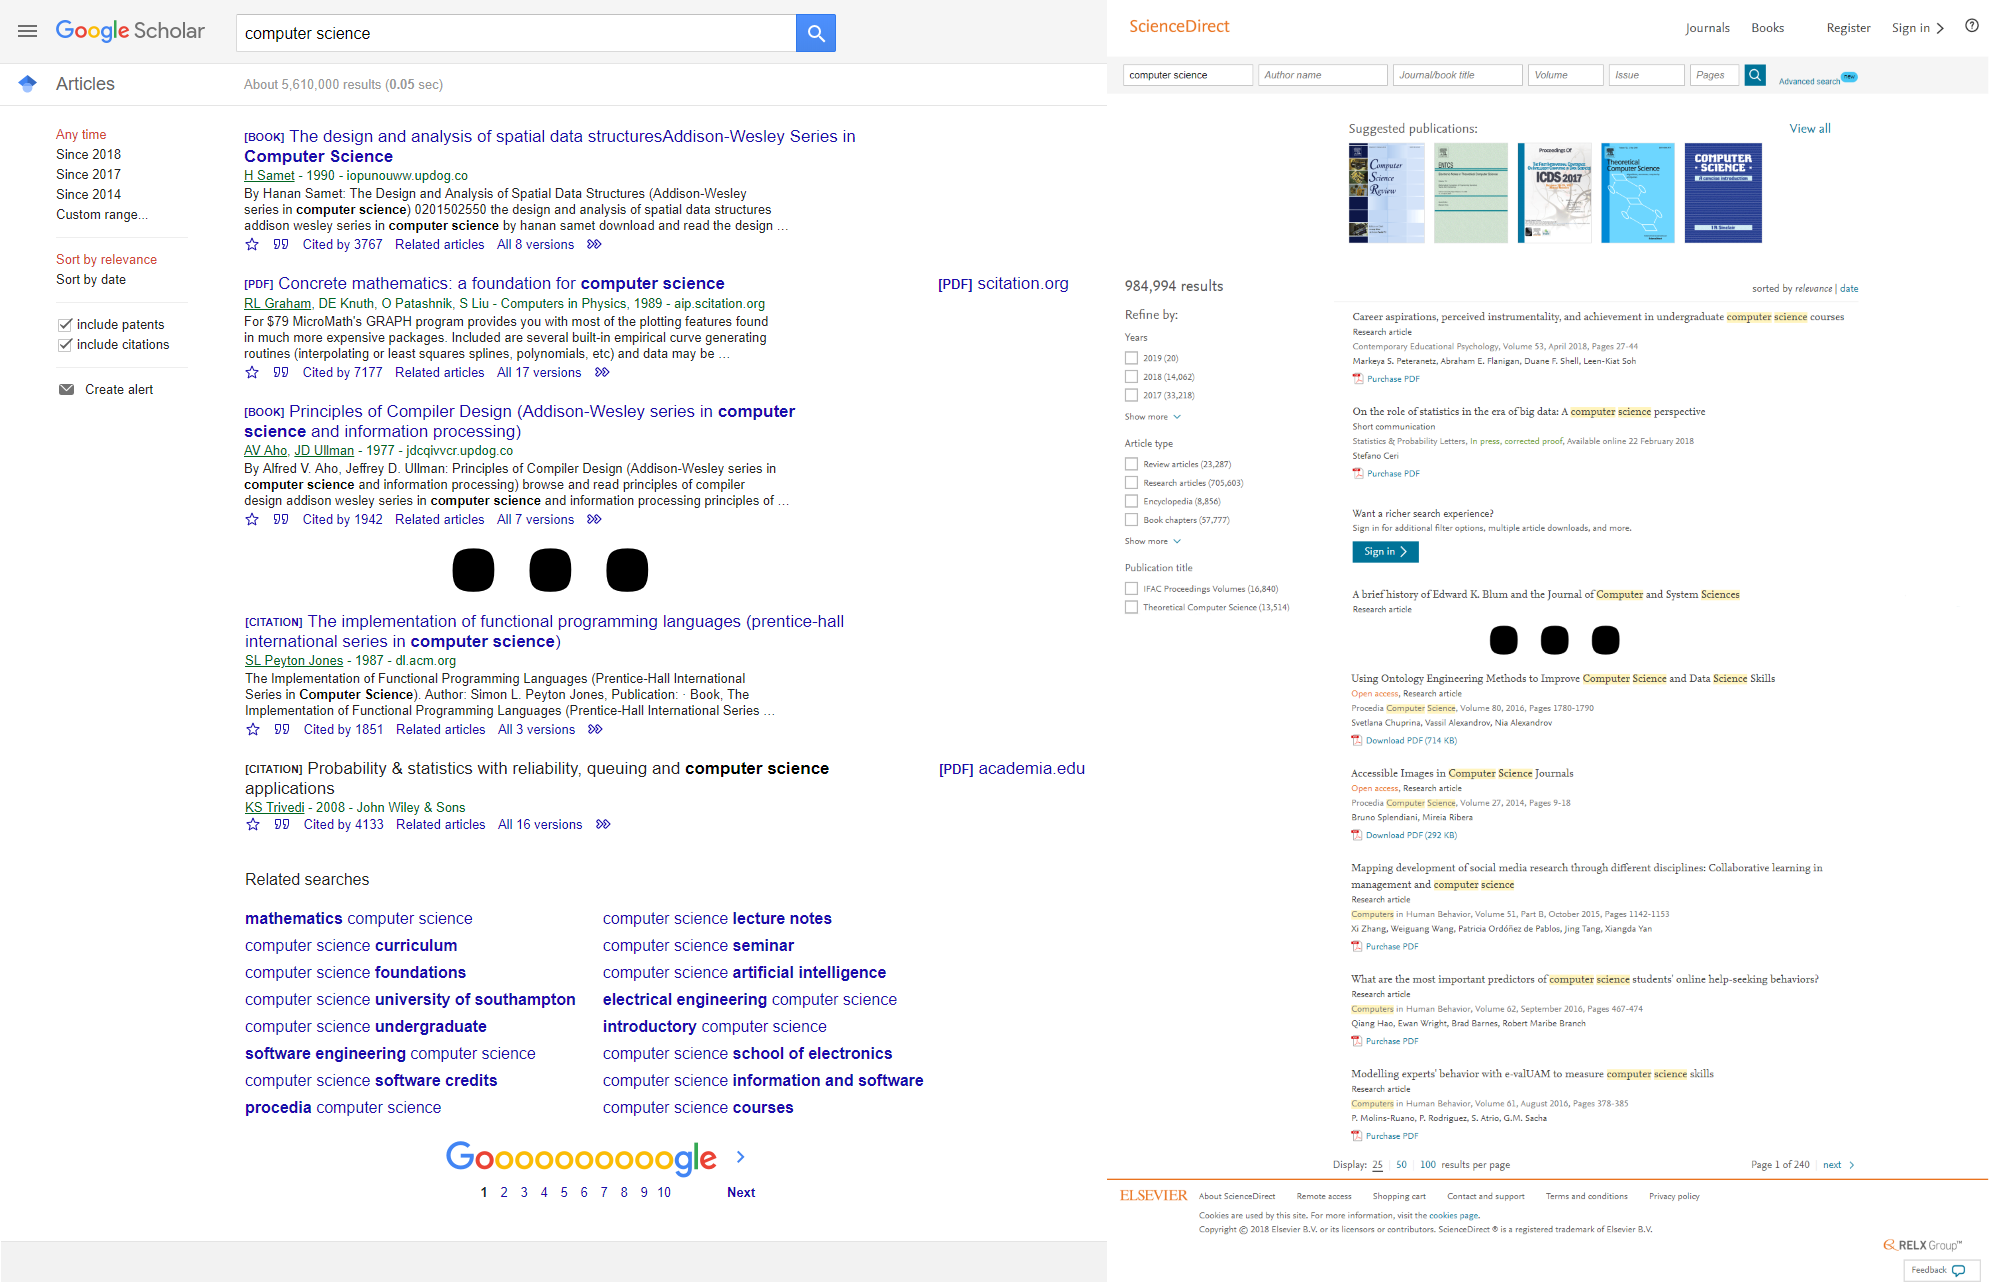
\includegraphics[width=\textwidth]{img/searchexamples.png}

\chapter{How to run the project from source}
\label{appendix:howtorun}

\end{appendices}

\end{document}
